\documentclass[
	dbse, 		 % include logo of DBSE working group
    %draft,    % omit title page, listings, and particular chapters selected below using include only
	%german,   % titles for a thesis in German, A4 paper
	%print,    % the printed version does not use colored links
	final,    % removes all TODOs
	a4paper   % forces A4 format even if <german> is not selected (useful for printing)
]{tex/ttthesis}

% Color Scheme http://colorschemedesigner.com/#3w40I--ALK-K-
% Base Color of the OVGU INF logo, tetraed, -45
\definecolor{blue1}{RGB}{0,105,180} % gray 95
\definecolor{blue2}{RGB}{40,87,121}
\definecolor{blue3}{RGB}{0,57,97}
\definecolor{blue4}{RGB}{76,166,230}
\definecolor{blue5}{RGB}{136,191,230}
\definecolor{orange1}{RGB}{255,144,0} % gray 133
\definecolor{orange2}{RGB}{171,121,56}
\definecolor{orange3}{RGB}{137,78,0}
\definecolor{orange4}{RGB}{255,181,84}
\definecolor{orange5}{RGB}{255,210,151}
\definecolor{green1}{RGB}{11,215,0} % gray 75
\definecolor{green2}{RGB}{52,144,48}
\definecolor{green3}{RGB}{6,116,0}
\definecolor{green4}{RGB}{88,241,80}
\definecolor{green5}{RGB}{148,241,143}
\definecolor{red1}{RGB}{253,0,6} % gray 86
\definecolor{red2}{RGB}{170,56,59}
\definecolor{red3}{RGB}{136,0,3}
\definecolor{red4}{RGB}{254,84,88}
\definecolor{red5}{RGB}{254,151,154}

\definecolor{background}{named}{white}
\definecolor{bgborder}{named}{black}
\definecolor{comment}{named}{red3}

\definecolor{blue}{named}{blue1}
\definecolor{green}{named}{green1}
\definecolor{red}{named}{red1}
\definecolor{orange}{named}{orange1}

\definecolor{pdflinkcolor}{named}{blue3}
\definecolor{pdfcitecolor}{named}{green3}

\usepackage{listings} % source code listings

%\renewcommand\lstlistingname{Quelltext}

\lstdefinestyle{java}{
%code formatting
	language=Java,
	tabsize=4,
	breaklines=false,
	basicstyle=\fontfamily{pcr}\footnotesize\selectfont,
	commentstyle=\fontshape{it}\color{darkgray}\selectfont,
	keywordstyle=\fontseries{b}\selectfont,
	stringstyle=\fontfamily{cmr}\selectfont,
%line numbering
	numbers=left,
	numberstyle=\footnotesize,
%frame properties
	captionpos=b,
	frame=single,%trblTRBL
	framesep=3pt,
	xleftmargin=4pt,
	xrightmargin=4pt,
	rulecolor=\color{bgborder},
}

\usepackage{pgfplots}
\usepackage{tikz}
	\usetikzlibrary{arrows,positioning,backgrounds,fit,trees} 
	\usetikzlibrary{fadings,shapes.geometric}
	\usetikzlibrary{decorations,scopes,calc,decorations.pathreplacing}

\ifgerman{
	\pgfplotsset{tick label style={/pgf/number format/1000 sep=.,/pgf/number format/use comma}}
}

% Tortendiagramme
\newcommand{\slice}[4]{
  \pgfmathparse{0.5*#1+0.5*#2}
  \let\midangle\pgfmathresult

  % slice
  \draw[thick,
	%fill=background
	] (0,0) -- (#1:1) arc (#1:#2:1) -- cycle;

  % outer label
  \node[label=\midangle:#4] at (\midangle:1) {};

  % inner label
  \pgfmathparse{min((#2-#1-10)/110*(-0.3),0)}
  \let\temp\pgfmathresult
  \pgfmathparse{max(\temp,-0.5) + 0.8}
  \let\innerpos\pgfmathresult
  \node at (\midangle:\innerpos) {#3};
}
\newcommand{\mypiechart}[2]{
	\begin{tikzpicture}[scale=#1]
		\newcounter{a}
		\newcounter{b}
		\foreach \p/\t in {#2}
			{
				\setcounter{a}{\value{b}}
				\addtocounter{b}{\p}
				\slice{\thea/100*360}
							{\theb/100*360}
							{\p\%}{\t}
			}
	\end{tikzpicture}
}

% surrounding TODOs with this command, gives you the ability to remove all if necessary
\iffinal{
	\newcommand{\todo}[1]{}
	\newcommand{\todots}{}
}{
	\newcommand{\todo}[1]{{\color{comment}\textit{[#1]}}}
	\newcommand{\todots}{\todo{\ldots}}
}

% propositional formulas
\newcommand{\pand}{\wedge}
\newcommand{\por}{\vee}
\newcommand{\pnot}{\neg}
\newcommand{\pequals}{\Leftrightarrow}
\newcommand{\pimplies}{\Rightarrow}
\newcommand{\pnimplies}{\nRightarrow}
\newcommand{\patmostone}{\mbox{\textit{atmost1}}}
\newcommand{\pchooseone}{\mbox{\textit{choose1}}}

% mathematical definitions and theorems
\newtheorem{definition}{Definition}[chapter]
\newtheorem{theorem}{Theorem}[chapter]
\newtheorem{lemma}{Lemma}[chapter]

% print URLs not in Typewriter Font
\def\UrlFont{\rm}

% empty page without page number, continue on the next right page
\newcommand{\blankpage}{\clearpage{\pagestyle{empty}\cleardoublepage}}

% index stuff
\makeatletter
\def\mydotfill{\leavevmode\xleaders\hb@xt@ .44em{\hss.\hss}\hfill\kern\z@}
\makeatother
\def\bold#1{{\bfseries #1}}
\newbox\dbox \setbox\dbox=\hbox to .4em{\hss.\hss} % dot box for leaders
\newskip\rrskipb \rrskipb=.5em plus3em % ragged right space before break
\newskip\rrskipa \rrskipa=-.17em plus -3em minus.11em % ditto, after
\newskip\rlskipa \rlskipa=0pt plus3em % ragged left space after break
\newskip\rlskipb \rlskipb=.33em plus-3em minus.11em % ragged left before break
\newskip\lskip \lskip=3.3\wd\dbox plus1fil minus.3\wd\dbox % for leaders
\newskip \lskipa \lskipa=-2.67em plus -3em minus.11em %after leaders
\mathchardef\rlpen=1000 \mathchardef\leadpen=600
\def\rrspace{\nobreak\hskip\rrskipb\penalty0\hskip\rrskipa}
\def\rlspace{\penalty\rlpen\hskip\rlskipb\vadjust{}\nobreak\hskip\rlskipa}
\let\indexbreak\rlspace
\def\raggedurl{\penalty10000 \hskip.5em plus15em \penalty0 \hskip-.17em plus-15em minus.11em}
\def\raggeditems{\nobreak\hskip\rrskipb \penalty\leadpen \hskip\rrskipa %
\vadjust{}\nobreak\leaders\copy\dbox\hskip\lskip %
\kern3em \penalty\leadpen \hskip\lskipa %
\vadjust{}\nobreak\hskip\rlskipa}
\renewcommand*\see[2]{\rlspace\emph{\seename}~#1} % from makeidx.sty


%*********************************************************************%
% META                                                                %
%*********************************************************************%

% available profiles: ovgu, tubs, tubs_isf
\ifgerman{
  \newcommand{\university}{Otto-von-Guericke-Universität Magdeburg}
  \newcommand{\school}{Fakultät für Informatik}
}{
  \newcommand{\university}{Otto-von-Guericke-Universität Magdeburg}
  \newcommand{\school}{Faculty of Computer Science}
}
\newcommand{\logo}{
\includegraphics[trim=0mm 0mm 50mm 0mm,clip,height=3cm]{INF_SIGN_druck}\ifdbse{\\[0.4cm]
  \logodbse}{ }}
\newcommand{\logodbse}{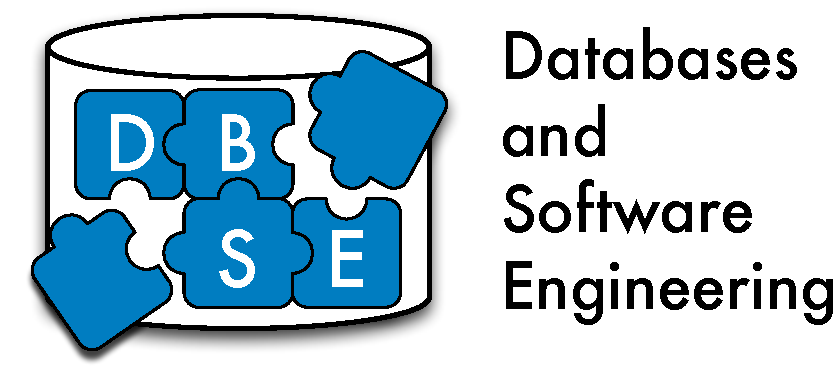
\includegraphics[scale=.45]{DBSE}}

\newcommand{\signatureplace}{Magdeburg}

\newcommand{\advisorone}{Dr.Ing {Eike Schallehn}}
%\newcommand{\advisortwo}{M.SC. Xiao Chen}
\newcommand{\departmentone}{Workgroup Databases and Software Engineering}


% Thesis kind
\ifgerman{\newcommand{\thesiskind}{Masterarbeit}}{\newcommand{\thesiskind}{Master's Thesis}}
%\ifgerman{\newcommand{\thesiskind}{Bachelorarbeit}}{\newcommand{\thesiskind}{Bachelor Thesis}}
%\newcommand{\thesiskind}{Diplomarbeit} %do not translate
%\ifgerman{\newcommand{\thesiskind}{Doktorarbeit}}{\newcommand{\thesiskind}{Dissertation}}

\ifgerman{
	\newcommand{\theforename}{\todo{Vorname}}
	\newcommand{\thesurname}{\todo{Nachname}}
	\newcommand{\thetitle}{\todo{Titel der Arbeit}}
	\newcommand{\thedate}{\todo{13. Monat 2014}}
}{
	\newcommand{\theforename}{Dharani Kumar}
	\newcommand{\thesurname}{Pasumarthi}
	\newcommand{\thetitle}{Evaluating the Efficiency of Parallel Semantic Document Matching using Apache Spark}
	\newcommand{\thedate}{May 3, 2018}
}
\newcommand{\theyear}{2018}
%date for signature in erklaerung.tex (declaration of originality)
\newcommand{\signaturedate}{03 May 2018}

%*********************************************************************%
% SETUP                                                               %
%*********************************************************************%

% meta informations of the document
\hypersetup{
 pdfauthor={\theforename\ \thesurname},
 pdftitle={\thetitle}
}

% open index file
\ifnotdraft{\makeindex}

%*********************************************************************%
% ACRONYMS                                                            %
%*********************************************************************%

% HOWTO: \gls{IDE} for singular or \glspl{IDE} for plural with 's
%\makeglossaries
\newacronym{IDE}{IDE}{Integrated Development Environment}
%\glsaddall % use only if you have acronyms that occur only in graphics

%*********************************************************************%
% THE DOCUMENT                                                        %
%*********************************************************************%

\begin{document}

\ifgerman{
	\labelformat{lstlisting}{Quelltext~#1}
	\renewcommand{\lstlistingname}{Quelltext}
}{
	\labelformat{lstlisting}{Listing~#1}
}

% set the path where graphics are located
\graphicspath{{pics/}}

\ifnotdraft{
	\frontmatter
	\pagenumbering{roman}
	\newcommand{\theauthor}{\theforename\ \thesurname}
\newcommand{\theauthorr}{\thesurname,\ \theforename}
\begin{titlepage}
 \thispagestyle{empty}
 \begin{center}
  {\university}\\[0.4cm]
  {\school}\\[2.0cm]
   \hbox{}\hfill
    \begin{minipage}[t]{\textwidth}
      \begin{center}
        \logo
	  \end{center}
    \end{minipage} 
   \hfill\hbox{}
  \ \\[0.4cm]
  \ifdbse{
  {\large \thesiskind \\[1cm]}
  {\huge\bf \thetitle \\[1cm]}
  }
  {
  {\large \thesiskind \\[1.6cm]}
  {\huge\bf \thetitle \\[1.6cm]}
  }
  { \ifgerman{Autor:}{Author:}}\\[0.4cm]
  {\huge \theauthor}\\[0.8cm]
  {\large\thedate}\\[0.8cm]
  {\ifgerman{Betreuer:}{Advisor:}}\\[0.4cm] 
  {\large
\advisorone
  }\\[0.2cm]
   {\large
%\advisortwo\ 
% }\\[0.2cm]
%  {
\departmentone
  }\\[0.8cm]
%  {\large
%\advisortwo\ 
 % }\\[0.2cm]
%  {
%\departmenttwo\ 
%  } 
 \end{center}
\end{titlepage}

%%%%%%%%%%%%%%%%%%%%%%%%%%%%%%%%%%%%%%%%%%%%%%%%%%%%%%%%%%%%%%%%%%%%%%%%%%%%
%%% Titelrückseite: Bibliographische Angaben
%%%%%%%%%%%%%%%%%%%%%%%%%%%%%%%%%%%%%%%%%%%%%%%%%%%%%%%%%%%%%%%%%%%%%%%%%%%%

\thispagestyle{empty}
\vspace*{\fill}
\begin{minipage}{15.0cm}
\textbf{\theauthorr:}\\
\emph{\thetitle\\}
\thesiskind, \university, \theyear.
\end{minipage}
\newpage

	\ifgerman{\chapter*{Inhaltsangabe}}{\chapter*{Abstract}}

In the cloud and web based scenarios, the volume of the documents from various platforms like digital libraries, news articles, and online forums etc are increasing at quick pace. It is a challenging task to efficiently process this magnitude of documents. The complexity would be of much greater scale if the process also involves in matching the documents based on their semantics. In this thesis, we have implemented a process flow for matching the similar documents based on the semantics using Latent Dirichlet Allocation (LDA) techniques. LDA techniques model a document into a distribution of topics by discovering the latent structure of the document along with the word occurrences. The semantic similarity is calculated by the information gained from a large corpus. As various approaches focused on increasing the efficiency of the Latent Dirichlet Allocation technique using MapReduce based and MPI based distributed environments, the entire Semantic Document Matching process is implemented using components of Apache Spark framework. Apache Spark is an open source, parallel processing engine to compute large amounts of data. The primary goal of the thesis is focused on increasing the efficiency of the Semantic Document Matching process. Additionally, we have calculated the effectiveness of the implemented process. Different experiments are performed on various sizes of a dataset in order to evaluate the Semantic Document Matching process.

	\blankpage
	
	\chapter*{Acknowledgements}
    Firstly, I would like to thank Dr. Eike Schallehn for providing me an opportunity to work under him and for his advise, encouragement throughout this thesis.
    \par I would also like to thank M.sc Xiao Chen and M.sc Yang Li for their assistance in answering all my queries.
    \par I would also thank Prof. Dr.-Ing. Andreas Nürnberger for spending time of his busy schedule to review my thesis. 
    \par This accomplishment would not be possible without my uncle's Narayana Rao, Srinivas. I am grateful to them for believing in me and supported certainly from day one.
    \par I thank my family and friends for their love and support.
	%\ldots 
	\blankpage
    
    \chapter*{Declaration of Academic Integrity}
    I hereby declare that this thesis is solely my own work and I have cited all external sources used.
\newline
\par\textit{Magdeburg, \(03^{rd}\) May 2018}


\begin{tabular}{p{0.45\textwidth}cp{0.45\textwidth}}
   \cline{3-3} \\
   & & \centering \textbf{Dharani Kumar Pasumarthi} 
\end{tabular}
    \blankpage
}

%*********************************************************************%
% LISTINGS                                                            %
%*********************************************************************%

\ifnotdraft{
	{\parskip 0pt \pdfbookmark{\contentsname}{\contentsname}\chapterheadfont \tableofcontents} % toc bitte einzeilig
	\blankpage

	\ifgerman{
		\listoffigures
		\addcontentsline{toc}{chapter}{Abbildungsverzeichnis}

		\listoftables
		\addcontentsline{toc}{chapter}{Tabellenverzeichnis}

		\renewcommand{\lstlistlistingname}{Quelltextverzeichnis}
		\blankpage
		\lstlistoflistings
		\addcontentsline{toc}{chapter}{\lstlistlistingname}

		%\renewcommand*{\firstacronymfont}[1]{\emph{#1}}
		%\printglossary[type=acronym,title=List of Acronyms,toctitle=Abkürzungsverzeichnis]
	}{
		\listoffigures
		\addcontentsline{toc}{chapter}{List of Figures}

		\listoftables
		\addcontentsline{toc}{chapter}{List of Tables}

		\renewcommand{\lstlistlistingname}{List of Code Listings}
		\blankpage
		\lstlistoflistings
		\addcontentsline{toc}{chapter}{\lstlistlistingname}

		%\renewcommand*{\firstacronymfont}[1]{\emph{#1}}
		%\printglossary[type=acronym,title=List of Acronyms,toctitle=List of Acronyms]
	}
}

%*********************************************************************%
% CHAPTERS                                                            %
%*********************************************************************%

\mainmatter
\pagenumbering{arabic}

\ifgerman{\chapter{Einführung}}{\chapter{Introduction}}
\label{introduction}
%- Hintergrund
%- Motivation
%- Ziele
%- Aufgaben
%- Allgemeine Beschreibung des Projektes
%- Worum geht es in dieser Arbeit?
%- Wer hat die Arbeit veranlasst und wozu?
%- Wer soll von den Ergebnissen profitieren?
%- Welches Problem soll gelöst werden? Warum?
%- Unter welchen Umständen braucht man eine Verbesserung?
%- Was ist der Stand der Technik?
%- Welche noch offenen Probleme gibt es?
%- Worin unterscheidet sich mein Ansatz von den bisherigen?
%- Welche Ziele hat die Arbeit?
%- Wie will ich diese Ziele erreichen?
%- Was habe ich im Einzelnen vor?

In the age of the digital world, the volume of the data is increasing exponentially day to day. Processing of the huge amount of documents in an efficient manner is becoming challenging and detecting the documents that are semantically similar within these huge data collections comes with various problems as the data needs to be converted to feature vectors representation. The problem arises because the feature vector are represented as sparse vectors and can be very high dimensional which requires high computational utilization.

\par One of the generally addressed approaches is to resolve the above mentioned problem by including the dimensionality reduction techniques in which the dimensions of the feature vectors are reduced without any data loss. But as the feature vector representation is only reliable on word occurrences, it can not be used for comparing documents based on semantic similarity. 

\par With the Latent Dirichlet Allocation (LDA) techniques along with the word occurrences, the structure of the document can also be considered. But the LDA techniques constitutes high intensive computations which can not be handled by a single computational machine. Hence, the process required to be implemented in a distributed environment. The distributed environment consists of several machines that are connected with each other and the task is divided among the machines resulting in parallel processing.

\par As MapReduce based implementations are already existing, we aspired to implement the parallel semantic document matching application using the Apache Spark ecosystem. Apache Spark is an open source, an in-memory data processing engine for faster computations \cite{spark:website}. The advantage with the Apache Spark is that the speed as it process majority of the computation in-memory.

\newpage
\paragraph{Goal of this Thesis}

The major goal of the thesis is to implement an application that compares any two documents in a corpus and find the similarity between them based on the semantics with in the Apache Spark framework. Also, to evaluate the efficiency and effectiveness of the application using diverse performance metrics.

\par The following tasks are carried out in progress of attaining the goal:

\begin{itemize}
\item The design and implementation of parallel semantic document matching application is developed. The application primarily encompasses six stages includes pre-processing, Count Vectorizer, LDA Modeling, Document pair comparison, classification, and evaluation. Using components from Apache Spark, all these stages are implemented.

\item To asses the application in a parallel environment, evaluations are carried out in terms of runtime performance, speed-up and efficiency. Additionally, to evaluate the quality of the results, measures like precision, recall and F-measure are also calculated. All these assessments are carried out on different sizes of datasets. 
\end{itemize}



\paragraph{Structure of the Thesis}

This thesis has been structured in the following format:

\begin{itemize}
\item \ref{introduction} provides an insight into the motivation and goals of the thesis.

\item \ref{background} is structured to provide the in-detail bedrock information required to understand the thesis as well as provides information on the related work in the fields of Latent Dirichlet Allocation (LDA) and document matching.


\item In \ref{concept}, we provide the information about the idea and the concept associated in developing the spark based semantic document matching application. 

\item \ref{implementation} discusses the process of implementation of this thesis.

\item In \ref{evaluation}, we discuss the results achieved by performing the evaluations.

\item In \ref{conclusion}, we conclude the thesis by presenting the experimental findings achieved on performing various experiments.

\item The possible areas of directions where the thesis can be extended is discussed in \ref{futurework}.
\end{itemize}


\ifgerman{\chapter{Grundlagen}}{\chapter{Background and Related Work}}
\label{background}
This chapter is structured to provide readers detailed insights of fundamental information required to understand this thesis. \ref{section: document matching} presents the bedrock concepts about document matching, applications and their necessity in the present world. In \ref{section: rcv1}, we provide a glimpse of our input dataset structure and its statistics. The process of document matching and its in-detail insights are illustrated in \ref{section: process of document matching}. Later, a brief introduction to  MapReduce and its limitations are discussed in \ref{section: Mapreduce}. In \ref{section: apache spark}, the concepts of Apache Spark framework that includes insights from basics to in-detail explanations of the ecosystem are emphasized. In \ref{section: Related work}, we discuss the previously implemented related work in the areas of document matching and Latent Dirichlet Allocation (LDA).

\section{Document Matching}
\label{section: document matching}
In the present realm of web-based and cloud-based technologies, the volume of the documents ranging from world wide web (WWW), online forums, digital libraries to news articles is increasing at rapid pace. On one hand processing this magnitude of documents efficiently is a challenging task and on the other hand, matching these documents by means of semantics would be of much more greater scale. 


\par  A corpus is a large collection of documents. In corpus based similarity, semantic similarity is carried out by measuring the similarity between documents with the help of information attained from the large corpora \cite{gomaa2013survey}. Within a Corpus, the problem of extracting similar documents based on their semantics has been broadly addressed by information retrieval community.

\par A subset of such addressing is based on the extraction of feature vectors from documents. The process starts by extracting feature vectors (words) from documents and then weighted by means of term frequencies (TF-IDF) which in turn produces a sparse vector and ends by comparing the documents in these sparse distances. But there are two problems associated with this process, one is the representation of feature vectors as sparse vectors. As these sparse vectors can be high dimensional which may require greater computational power. Additionally, the size of the feature vector increases with increase in the length of the document. Hence the approach is appreciable for fixed length document. The other is that the TF-IDF approach is reliable on only word occurrences which may not give desirable results if two documents are having the same context but are expressed with different representations or different words. For Example, consider the following two news articles published by two different newsgroups :
\newline

Article 1: A gigantic cyclone hit the southern part of Germany. 
\newline
\par Article 2: Eventually, part of Germany was stormed by the hurricane on a massive scale.
\newline
\par From the above two articles, we can observe that the two articles are speaking about the same information contextually but expressed in different terms. This is the major limitation of any approach that uses TF-IDF though the problem of high dimensionality is addressed by various dimensionality reduction algorithms. 

\par We try to describe an implementation which involves in addressing the above stated problems such as match documents irrespective of its contained length. Instead of just relying on word occurrences, our implementation additionally considers the structure of the document. Also, we implemented our application using the parallel environment to process a huge volume of documents as our primary focus is on reducing execution time and are discussed in consecutive sections.


\subsection{Applications}
In this section, some of the examples that are used for document matching application are illustrated in the following:

\begin{itemize}
\item \textbf{Help Desk Application:} Help-desk in any institute or organization plays a vital role in helping their customers or users. The application is implemented to act as a response system. The focus of the application is to help its users to provide necessary information on problem description. A user has to input a problem description and the application takes that problem as a query and is compared to the entire corpus in order to provide the useful information to the user. For this purpose, document matching techniques are used \cite{weiss2000lightweight}.

\item \textbf{Literature Search Tool:} PubMed is a literature search tool developed by National Center for Biotechnology Information at United States National Library of Medicine. The literature consisting of over 28 million citations. The tool provides results based on the keywords provided to the query. The available literature covers a range of biomedical, health, chemical sciences, bioengineering to life sciences. For any given query, the search engine of the PubMed tool produces results based on the document pair similarity scores \cite{website:pubmed}. 
\end{itemize}


\newpage
\section{Reuters Corpus Version 1}
\label{section: rcv1}

\begin{figure}[hp]
	\centering
		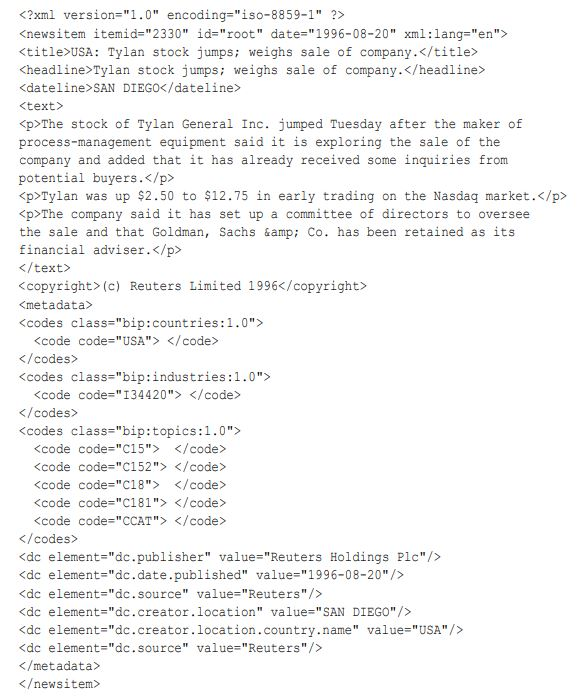
\includegraphics[scale=1.00]{Reutersdoc}
	\caption{A sample document from Reuters Corpus Version 1 \cite{lewis2004rcv1}}
	\label{fig:reutersdoc}
\end{figure}

The dataset that we used as input is Reuters Corpus Version 1 (rcv1). Rcv1 in total has 806,791 documents that are manually categorized news articles from Reuters Ltd. The contents of all the documents are in the English language. From the \ref{fig:reutersdoc}, it can be seen that the documents are produced in extensible Markup Language (XML) format and provides further sophisticated information about how a document is produced. The additional information about the corpus and document structure are discussed in the following \cite{lewis2004rcv1}:
\begin{itemize}
\item Every document consists of unique document ID and range from 2286 to 810597. In \ref{fig:reutersdoc}, the document id can be found as itemid in between the tags named newsitem. This unique Document ID is used for the entire document matching process.

\item From \ref{fig:reutersdoc}, the data in between the tags named text is the news article that is providing information about the specific context where <p> represents a paragraph. The whole data in between text is required for the process of document matching.  

\item  All the documents in the corpus are divided into three categories namely Topics, Industries, and Regions.

\item A total of 103 codes are available under topics and the assignment of the topic to a document is performed within these codes. A document can have no assignment, a single assignment or multiple assignments of codes. The assignment of codes was performed automatically but under the supervision of human editors. In \ref{fig:reutersdoc}, the assignment of the various topics to a single document can be seen in between the tags codes that point to the class bip:topics:1.0

\item The document also provides an additional metadata information such as copyright that a document belongs to, the origin of document or news article generated, the date that news article published etc.
\end{itemize}
  
\par For evaluation purposes, We have chosen Reuters corpus as we need a large amount of documents in order to evaluate the parallel performance and scalability of our application. The corpus does not possess any information or labels that represent the semantic relation between two documents which can be in short called as the ground truth table. Hence we have implemented a work around method to generate gold standard data and is used for effectiveness evaluations. The detail description of the workaround method is discussed in \ref{implement:evaluation}.


\section{Process of Document Matching}
\label{section: process of document matching}

\begin{figure}[htp]
	\centering
		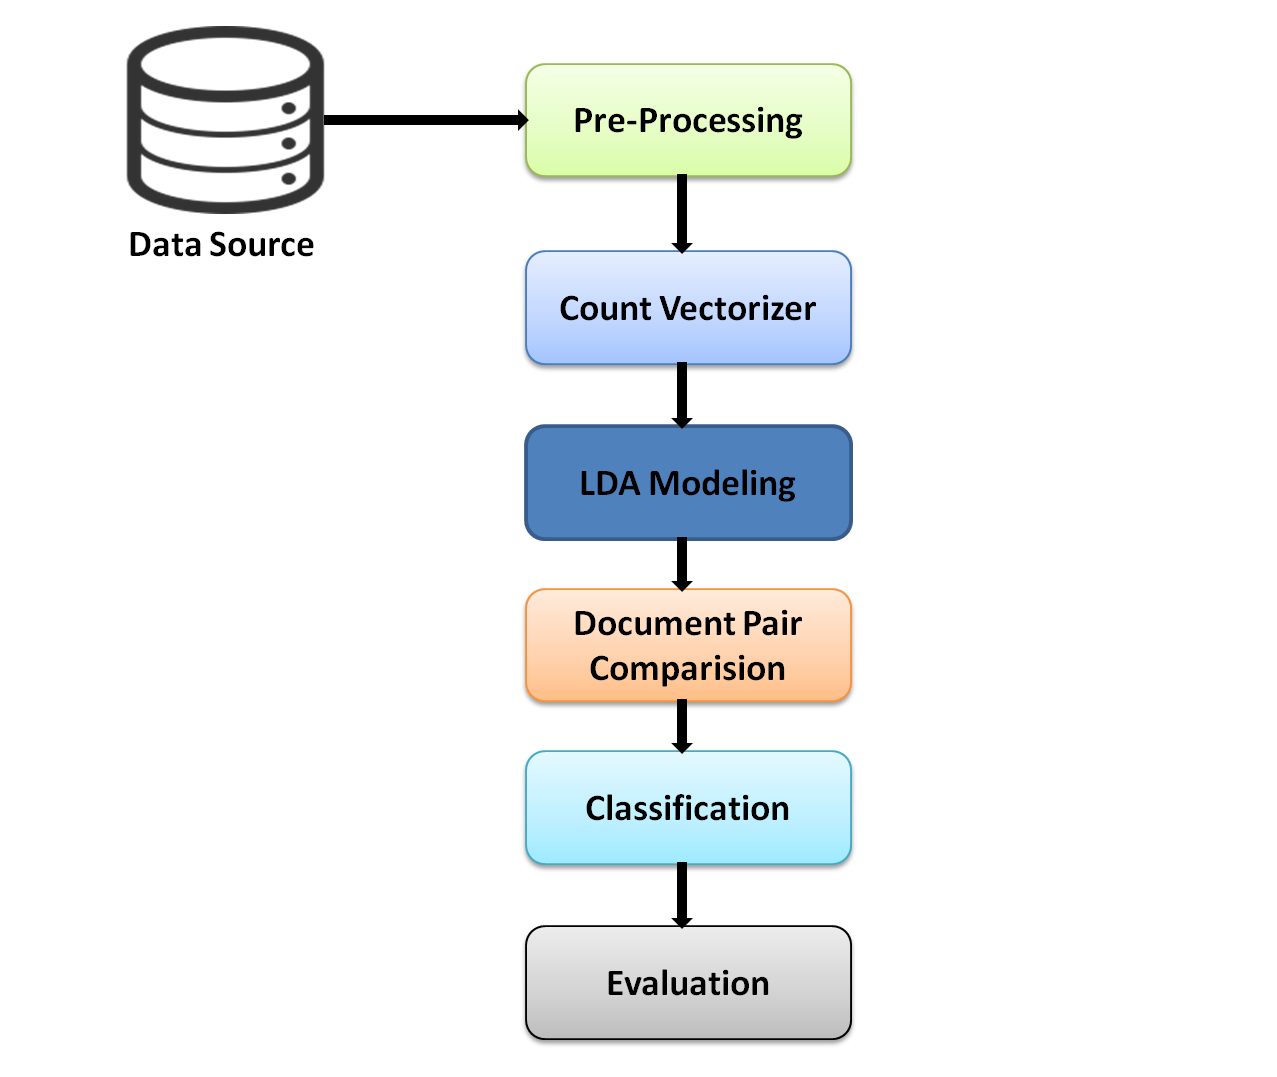
\includegraphics[scale=0.60]{Process}
	\caption{Work flow of Document matching process}
	\label{fig:process}
\end{figure}

As illustrated in the \ref{fig:process}, the implementation of the Document Matching involves six major stages namely pre-processing, count vectorization, Modeling, Document pair comparison, Classification, and Evaluation. The detailed information provided in the following sections improves ones understanding of the document matching process. \ref{section: preprocessing} provides information on the requirement of a pre-processing stage. A document is required to be represented in sparse vectors for any algorithm to understand and are discussed in detail in \ref{section: countvectorizer}. Once a document is represented in a sparse vector, it is then sent to document modeling algorithm for the purpose of document matching and \ref{section: lda} provides detailed insights. To find which documents are matching semantically, every document in the corpus is compared to other document and the logical theory behind it is discussed in \ref{section: document pair comparison}. In the classification stage, the compared documents are classified as match or non-match and the classification techniques used for the purpose are explained in \ref{section: classification}. Finally, the output from the classification stage is sent to the last stage called evaluation stage where certain evaluation schemes are used and are elucidated in \ref{section: evaluation}.


\subsection{Pre-processing}
\label{section: preprocessing}
The first step of our implementation is pre-processing of data. As can be seen from \ref{fig:reutersdoc}, the data which we require is a document and is in XML structure and has to be cleaned and to be brought to a data format that is acceptable by the framework before initializing to any further steps. It is essential to filter out unwanted data otherwise it may lead to inaccurate computations which may finally results in inaccurate evaluations. Hence, it is mandatory to clean the data in order to increase the input data quality. Internally, this step is further divided into three phases consisting of parsing data, tokenization and stop words removal and are explained in the following:
\begin{enumerate}
\item \textbf{Parsing Data:} If the data is semi-structured and holds different kinds of information in the same document. It is required to separate and retrieve the relevant data fields from the irrelevant ones.

\item \textbf{Inferring Schema:} After the required data fields are extracted from the document, then we have to standardize the data fields according to the acceptable data format either by inferring schema implicitly or explicitly.

\item \textbf{Tokenizaton:} The process of breaking or splitting a sentence to a series of individual words is referred as tokenization. The individual words generated in this process can be called tokens. It is also obligatory to remove special characters such as `,' , `<' ,`\' , `?' etc as these characters do not possess any useful information in the process of document matching.

\par For example, let us consider two sentences and observe how a tokenization process extract tokens and is illustrated in \ref{tab:tokenization process example}.

\begin{table}[htbp]
	\centering
		\begin{tabular}{ccc}\toprule
			& Input & Output\\\midrule
		Sentence 1 & Hello! < how are you?> & [ hello, how, are, you ]\\\addlinespace 
		Sentence 2 &  I love to travel countries & [ i, love, to, travel, countries ] \\\addlinespace
			\bottomrule
		\end{tabular}
	\caption{An Example of tokenization process}
	\label{tab:tokenization process example}
\end{table}



\item \textbf{Stop Words Removal:} The words that frequently appear in the data and doesn't hold neither useful information nor influence of meaning on the document is referred as stop words \cite{fox1989stop}. Some of the stop words include I, the, is, a etc. As these words have no significance, these words are to be removed from the data.

\par An example is illustrated in \ref{tab:stopwords process example}.

\begin{table}[htbp]
	\centering
		\begin{tabular}{ccc}\toprule
			& Input & Output\\\midrule
		Sentence 1 & The dog is a good pet & [ dog, good, pet ]\\\addlinespace 
		Sentence 2 &  I wish  to travel the world & [ wish, travel, world ] \\\addlinespace
			\bottomrule
		\end{tabular}
	\caption{An Example of stop words removal process}
	\label{tab:stopwords process example}
\end{table}


\end{enumerate}


\subsection{Count Vectorizer}
\label{section: countvectorizer}
In our application, after cleaning of the input data, A document has to be converted to vector representation for further processing and can be performed using Count Vectorizer. The numerical values generated inside the vector by Count Vectorizer represents the influence of a single word that has with the particular document in the Corpus. Count Vectorizer builds a matrix that is sparse in nature based on the word occurrence of each document in the corpus. The matrix consists of documents over Vocabulary. Count Vectorizer maintains a dictionary in which the unique words are stored and compared.  For example, we presume that we have four different documents containing respective sentences as illustrated in  \ref{tab:documents and sentences}.

\begin{table}[htbp]
	\centering
		\begin{tabular}{cc}\toprule
			Document & Sentence\\\midrule
			1 & Hello How are you\\\addlinespace 
			2 &  How do you do\\\addlinespace
			3 & Where are you\\\addlinespace
            4 & Where you been\\\addlinespace
			\bottomrule
		\end{tabular}
	\caption{Documents containing sentences}
	\label{tab:documents and sentences}
\end{table}

\par Firstly the process of Count Vectorizer starts by creating a dictionary of unique words that it recognizes from documents. An unique ID is assigned to every unique word and the dictionary for documents \ref{tab:documents and sentences} is illustrated in \ref{tab:dictionary}.

\begin{table}[htbp]
	\centering
		\begin{tabular}{cc}\toprule
			ID & Word\\\midrule
			1 & Hello \\\addlinespace 
			2 &  How  \\\addlinespace
			3 & are\\\addlinespace
            4 & you \\\addlinespace
            5 & do \\\addlinespace
            6 & Where \\\addlinespace
            7 & been \\\addlinespace
			\bottomrule
		\end{tabular}
	\caption{Dictionary by Count Vectorizer }
	\label{tab:dictionary}
\end{table}

\par The dictionary in \ref{tab:dictionary} represents that a total of seven distinct words found by the Count Vectorizer for four documents respectively.

\par Now by considering the dictionary, the Count Vectorizer generates a matrix by mapping the presence of feature along with times the feature appeared in that particular document as shown in \ref{tab:Document vocabulary Matrix}. From the \ref{tab:Document vocabulary Matrix}, we can observe that every 1 represents the occurrence of a feature that appeared in the particular documents whereas 0 states the absence of that particular feature in that document. The count of the particular feature is proportional to the number of times the feature appears in the particular documents and the same can be observed within document 3.


\begin{table}[htbp]
	\centering
		\begin{tabular}{cccccccc}\toprule\addlinespace
			 & Feature 1 & Feature 2 & Feature 3 & Feature 4 & Feature 5 & Feature 6 & Feature 7\\\addlinespace\midrule
			Document 1 & 1 & 1 & 1 & 1 & 0 & 0 & 0 \\\addlinespace
       
			Document 2 &  0 & 1 & 0 & 1 & 2 & 0 & 0 \\\addlinespace
            
			Document 3 & 0 & 0 & 1 & 1 & 0 & 1 & 0\\\addlinespace
            
            Document 4 & 0 & 0 & 0 & 1 & 0 & 1 & 1\\
            \bottomrule
		\end{tabular}
	\caption{Document Vocabulary Matrix  generated by scheme of Count Vectorizer}
	\label{tab:Document vocabulary Matrix}
\end{table}

\par The final representation of the sparse vector generated by Count Vectorizer can be seen in \ref{tab:vector representation} where 7 represents the dictionary size, the second array represents the IDs of the appeared features in the particular document and third array represents the word occurrences of the particular feature.


\begin{table}[htbp]
	\centering
		\begin{tabular}{cc}\toprule
			  & Vector\\\midrule
		Document 1 & (7, [1,2,3,4], [1,1,1,1])\\\addlinespace 
		Document 2 &  (7, [2,4,5], [1,1,2])\\\addlinespace
		Document 3 & (7, [3,4,6], [1,1,1])\\\addlinespace
        Document 4 & (7, [4,6,7], [1,1,1])\\\addlinespace
			\bottomrule
		\end{tabular}
	\caption{Vector representation by Count Vectorizer}
	\label{tab:vector representation}
\end{table}

\subsection{Latent Dirichlet Allocation}
\label{section: lda}
This step is the heart of our application. It aims at building a document-topic matrix based on how a document can be expressed in terms of its context and is discussed in detail in the following.

\begin{figure}[htbp]
	\centering
		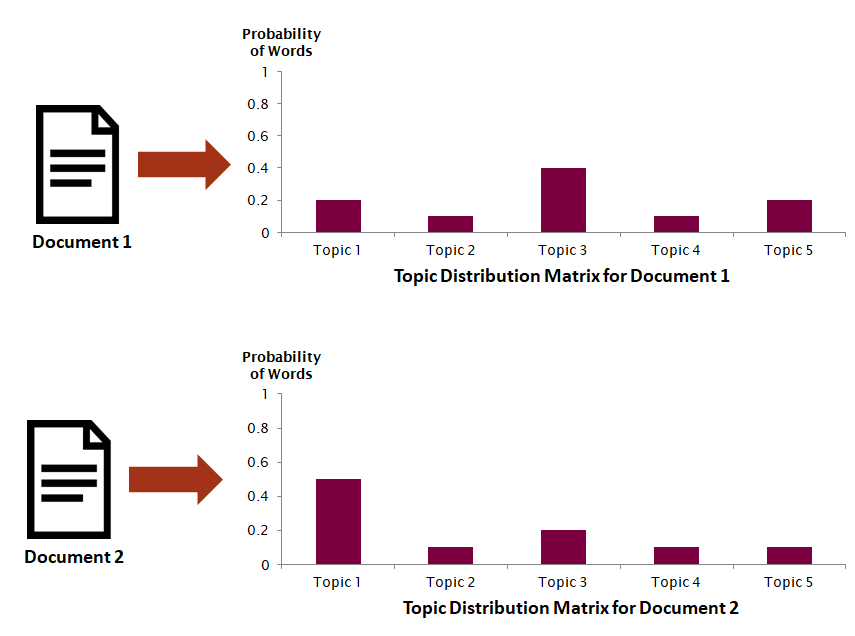
\includegraphics[scale=0.65]{lda}
	\caption{Representation of a sample documents in terms of 5 topics by Latent Dirichlet Allocation }
	\label{fig:lda}
\end{figure}

\par In 2003,  researchers David M. Blei, Andrew Y.Ng and, Michael I. Jordan first proposed a topic modeling algorithm for a large set of text documents referred as Latent Dirichlet Allocation (LDA). LDA is an unsupervised machine learning algorithm. LDA can also be used for context visualization and context summarization on huge voluminous document collections.  As illustrated in \ref{fig:lda}, LDA represents a document as a probabilistic distribution of topics where the axis named probability of words represents the total number of words contributing to the particular topic \cite{blei2003latent}. From \ref{fig:lda}, we can observe the different topic distributions for different documents.


\par LDA assumes that a document is produced or written with the following criteria:
\begin{itemize}
\item Every document is a probabilistic distribution of topics
\item Every topic is a probabilistic distribution of words
\end{itemize}

\par Based on the above assumptions, LDA observes the words in any given document and assigns a probability to each word that belongs to a topic finally resulting in topic distribution and can be seen in \ref{fig:ldacorpus}.
\begin{figure}[htbp]
	\centering
		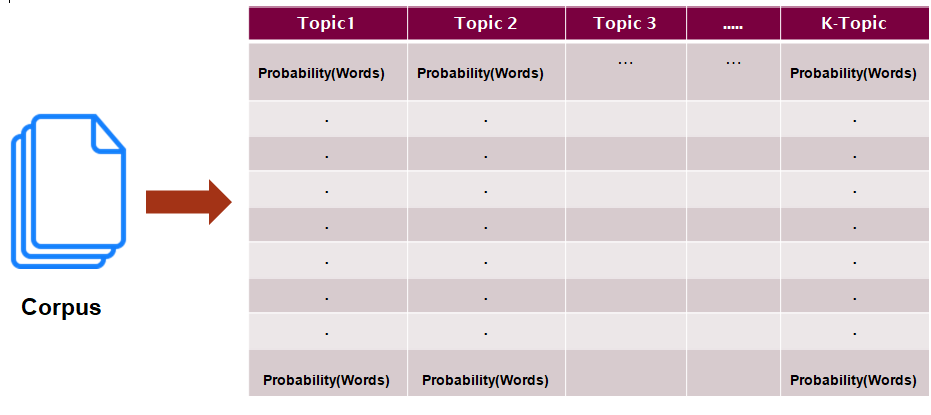
\includegraphics[scale=0.60]{ldacorpus}
	\caption{Representation of a corpus in terms of document topic matrix by Latent Dirichlet Allocation where each row of the matrix represents a document}
	\label{fig:ldacorpus}
\end{figure}


\par From \ref{fig:ldacorpus}, a corpus is a collection of the large set of documents. Each row represents a document and is represented by K latent topics. By this matrix, any two documents can be compared to calculate the semantic similarity between them as the documents are representing the structure or context. 

\par We have used the following learning algorithm for LDA to discover the topics and is discussed:

\textbf{Expectation Maximization:} 

Expectation Maximization algorithm contains two steps namely Expectation (E-step) and Maximization (M-step). The algorithm process these two steps iteratively. The work of the E-step is to infer the topic distribution of each document. Then the M-step updates the parameters of the model based on the inference result from the E-step \cite{blei2003latent,nallapati2007parallelized}. 

\par Apart from the above mentioned algorithm, there exist various other learning techniques used for LDA topic discovery. Some of them are Gibbs sampling method, Expectation Propagation Method, collapsed Gibbs sampling, Markov chain Monte Carlo method etc \cite{minka2002expectation,griffiths2004finding}.



\subsection{Document Pair Comparison}
\label{section: document pair comparison}
In this step of document matching, we compare two documents for similarity purpose. It is necessary to compare two documents to measure the semantic similarity between them. We used the following distance metric to validate the purpose.

\textbf{Hellinger distance metric:} In 1909, Ernst Hellinger introduced the Hellinger distance. Hellinger distance metric is used for measuring the distance between two probabilistic distributions since the documents after the LDA step are represented in probabilistic distributions. 

\par For example, let us consider two probabilistic distributions A = \( (a_1, a_2, a_3....a_n)\) and B = \( (b_1, b_2, b_3....b_n)\) then Hellinger distance for these probabilistic distribution is defined as

\begin{equation}\label{formula: hellinger equation}
H(A,B) = \frac{1}{\sqrt{2}}\sqrt{\sum{}_i^n(\sqrt{a}_i - \sqrt{b}_i)^2}
\end{equation}


\par The boundaries of Hellinger distance lies between 0 and 1. The lesser the value, the higher the two documents are similar and vice-versa \cite{gibbs2002choosing} \cite{rus2013similarity}.

\subsection{Classification}
\label{section: classification}
\par In this step, the compared two documents from the document pair comparison step are classified as match or non-match by the classification technique. We have used the following classification technique to justify the purpose. This step can also be called as a binary classification problem.

\textbf{Classification based on Threshold value:} To categorize the document pair as match or non-match, a threshold function is defined as \textit{Similarity} where it compares the scores of two documents that are obtained in the previous step. Let us consider a document pair \((d_i, d_j)\) which holds a similarity score calculated in the previous step. Now, let \textit{'alpha'} be the threshold value enforced on document pair  \((d_i, d_j)\)  then the document pair is classified based on the two following predicates:

\begin{equation}\label{formula: threshold value for match}
\textit{Similarity\((d_i, d_j)\)}   \leq   \textit{alpha}  \Rightarrow (d_i, d_j)  \text{ is a match}
\end{equation}

\begin{equation}\label{formula: threshold value for non-match}
\textit{Similarity\((d_i, d_j)\)}   >  \textit{alpha}  \Rightarrow (d_i, d_j)  \text{ is a non-match}
\end{equation}

\subsection{Evaluation}
\label{section: evaluation}
Evaluation is the final step of our application. In this step, we perform various evaluations on the application to calculate the parallel performance such as total execution time taken by the application. Therefore, the following metrics are used for calculating the performance \cite{wilkinson1999parallel}: 

\begin{itemize}
\item Speedup: If \(TT_1\) be the total execution time taken by the application to execute on single node and  \(TT_i\) be the total execution time taken on \textit{` i '} nodes in a clusters, then  the ratio of total execution time on single node to the total execution time on \textit{` i '} nodes is defined as Speedup `\(S_i \)' and is represented as following:

\begin{equation}\label{formula: speedup}
S_i = \frac{TT_1}{TT_i}
\end{equation}

\item Efficiency: In a parallel environment, Efficiency is calculated as a measure of computational power utilized by the processors while executing the application. Efficiency is directly proportional to Speedup and hence Efficiency `\(E_i\)' is represented as

\begin{equation}\label{formula: efficiency}
E_i = \frac{S_i}{i}
\end{equation}

 
\item Scale out: Scale out expresses the handling capacity of an application in managing the data growing with respect to cluster size that uses parallel processing. The execution time of an application should be constant irrespective of the increasing data and cluster size. 
\end{itemize}
 
\textbf{Effectiveness} 
\par In addition to the above evaluation metrics, the quality of the classified data can also be measured.  The correctness of data that has been classified according to the predicate can only be known by the golden standard data. The golden standard data posses information about the authentic matches and non-matches of the data. With the help of confusion matrix, the predicted labels can be compared to the true labels and have the following four categories \cite{tripathy2015classification}.

\begin{itemize}
\item True Positives (TP): The total document pairs positively predicted by the classifier as well as true in golden standard data.

\item False Positives (FP): The total document pairs positively predicted by the classifier but are false in golden standard data.

\item True Negatives (TN): The total document pairs predicted as negative by the classifier but are true in golden standard data.

\item False Negatives (FN): The total document pairs predicted as negative by the classifier as well as false in golden standard data.
\end{itemize}

\par Also, Using confusion matrix the quality based measures like precision, recall and, f-measures can be calculated. In the area of information retrieval, these measures are extensively used \cite{christen2007quality}. The respective formulations are listed below \cite{tripathy2015classification}:

\textbf{\textit{Precision:}} The ratio of a number of predictions that are correctly predicted (TP) to the total number of classifications (TP+FP) can be defined as Precision. With the help of Precision, the exactness of the classifier can be acknowledged \cite{tripathy2015classification}.

\begin{equation}\label{formula: Precision}
\textit{Precision} = \frac{TP}{TP+FP}
\end{equation}

\textbf{\textit{Recall:}} The ratio of a number of predictions that are correctly predicted (TP) to the total number of authentic positives (TP+FN) in the golden standard data can be defined as Recall. Recall can be used to acknowledge classifier in terms of completeness \cite{tripathy2015classification}.

\begin{equation}\label{formula: Recall}
\textit{Recall} = \frac{TP}{TP+FN}
\end{equation}

\textbf{\textit{F-Measure:}} F-measure is defined as the harmonic mean of the recall and precision. F-measure can also be referred as F-Score and is represented as \cite{tripathy2015classification}:


\begin{equation}\label{formula: F-Measure}
\textit{F-Measure} = 2 \times \frac{precision \times recall}{precision+recall}
\end{equation}

As F-measure is directly proportional to precision and recall, the high value of the F-Measure can be obtained by obtaining the better values of the precision and recall.


\section{MapReduce}
\label{section: Mapreduce}
To process huge voluminous data, on the idea of divide and conquer Google conferred a programming model named MapReduce. MapReduce is developed for parallel, distributed environments. Map and Reduce are the two basic functionalities offered by the MapReduce programming model to let specify by the users. The underlying data structure in MapReduce is Key/value pairs.When a user specifies the Map, the function takes the input data and yields a set of intermediate values in the form of key/value pairs. The MapReduce library then combines all the intermediate values having the same key. It is then passed as an input to the reduce function. The Reduce function then accept these intermediate values and then aggregates the values holding the same key. MapReduce offers for an application that requires scalability and tolerance \cite{dean2010mapreduce}. The programming model of the MapReduce is illustrated in \ref{fig: Mapreduce}.

\begin{figure}[htbp]
	\centering
		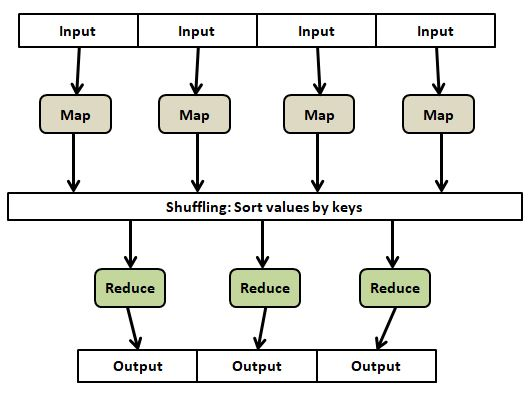
\includegraphics[scale=1.00]{Mapreduce}
	\caption{An illustration of MapReduce programming model based on \cite{elsayed2008pairwise}}
	\label{fig: Mapreduce}
\end{figure}

\par To define a function by a user, the following are the signatures provided as an abstraction by the MapReduce 
\cite{elsayed2008pairwise}:

\[Map: (Key1,Value1) \implies list(Key2,Value2)\]
\[Reduce: (Key2,list(Value2)) \implies list(Key3,Value3)\]


To process big data across multiple clusters based on the Google's MapReduce, Apache developed an open source framework referred as Apache Hadoop. The framework is developed for processing distributed and scalable computations. Hadoop Distributed File System (HDFS), Hadoop common, Hadoop YARN and Hadoop MapReduce are the major components offered by the Hadoop and are discussed in the following \cite{website:hadoop}:

\begin{itemize}
\item Hadoop Common: This module helps in the startup of the Hadoop by running the configuration scripts. Also, this module includes abstraction for operating systems and Java libraries.

\item Hadoop YARN: This module is responsible for scheduling of job tasks and management of resources across clusters. The management of resources is processed through node managers and resource managers by YARN. YARN abbreviates to Yet Another Resource Negotiator. 

\item Hadoop MapReduce: This component offers MapReduce programming model on YARN clusters for parallel processing of data sets of large scale.

\item Hadoop Distributed File System (HDFS): This component offers to store huge voluminous dataset through the distributed file system in a cluster. The advantage of this component is it to make sure that data is accessible by all nodes in the cluster. Hence, is suitable for large scale applications.

\end{itemize}


\textbf{Limitations}
\par Though MapReduce has many advantages for parallel processing of big data but shows inefficiency in performing computations for applications that use iterative algorithms as well as for interactive applications. Some of the reasons are stated below \cite{Jonnalagadda2016}:

\begin{itemize}
\item Because of writing and reading of inputs/outputs to and from disks, serialization, and replication, the data sharing between tasks are time consuming. Hence most of the applications allocate greater time in read-write operations.

\item The applications that use iterative algorithms often need data to be reused multiple times. When an iterative application is processed on MapReduce, the intermediate results in MapReduce programming model writes to disks on every iteration thereby causing an I/O communication overhead which can be seen in \ref{fig: iteration}.
\end{itemize}

\begin{figure}[htbp]
	\centering
		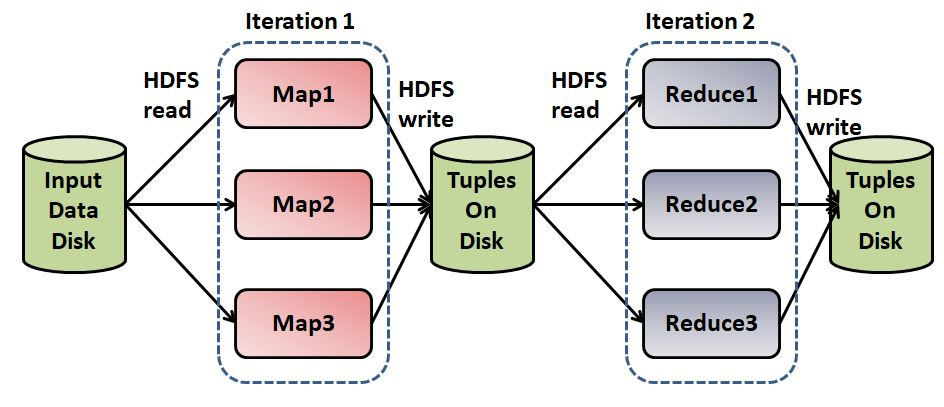
\includegraphics[scale=0.60]{Iteration}
	\caption{An Example of iteration process in MapReduce \cite{Jonnalagadda2016} }
	\label{fig: iteration}
\end{figure}



\section{Apache Spark}
\label{section: apache spark}
This thesis uses the Apache Spark framework to implement parallel processing of a large set of documents. Hence, this section provides the bedrock information about Apache Spark.

\par Apache Spark, an open source cluster computation engine for processing and analyzing huge voluminous data commonly referred as big data. It was initially developed by Matei Zaharia in 2009 at UC Berkeley's AMPLab \cite{Jonnalagadda2016}. It is a unified framework to support a variety of workloads including streaming, batch processing, iterative algorithms and interactive queries \cite{karau2015learning}. One of the fundamental highlights Spark offers for speed is the capacity to run computations in-memory. Another being tight-integration with other big data tools, accessibility of application programming interfaces (APIs) in various programming languages like Scala, Java, Python and R \cite{karau2015learning}. 

\par MapReduce and many of its versions use an acyclic data flow model and have been efficient in performing voluminous data-intensive applications on commodity clusters. But they are not appropriate for interactive data analytics, machine learning applications which uses algorithms that are iterative in nature and requires functional dataset to be reused across multiple parallel operations \cite{zaharia2010spark}. On surveying these drawbacks, researchers Matei Zaharia, Mosharaf Chowdhury, Michael J. Franklin, Scott Shenker and Ion Stoica presented a framework named Spark.
 
 
\par Spark works on in-memory cluster computation while preserving the properties such as scalability and fault tolerance of MapReduce \cite{zaharia2010spark}. Rather than loading of data from disk, Spark facilitates the machines to cache intermediate results and data in memory on each iteration. Thus, offering more space for efficiency in iterative computations and is appropriate for substantial scale machine learning applications \cite{bao2016large}.

\par  The primary idea on which Spark was build for distributed shared memory abstraction is adverted as Resilient Distributed Datasets (RDDs)  \cite{Zaharia2012}. In \ref{Spark Core}, the concept of RDDs is discussed in detail. 


\subsection{Traits of Spark}
Other traits apart from in-memory cluster computations of Spark are discussed in this section.
\begin{itemize}
\item \textbf{Swift Processing:} As spark benefits from in-memory caching, the computational performance of Spark in Hadoop clusters is 100 times swifter if run in memory and 10 times if run on disk when compared to Hadoop MapReduce\cite{spark:website}. For an identical application, the difference in runtime performance between Spark and Hadoop is illustrated in \ref{fig:runtime}

\begin{figure}[htbp]
	\centering
		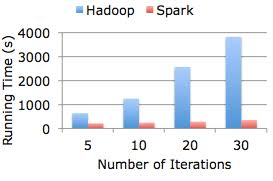
\includegraphics[scale=1.00]{runtime}
	\caption{Total runtime performance of logistic regression in Spark and Hadoop \cite{spark:website} }
	\label{fig:runtime}
\end{figure}

\item \textbf{State-of-the-art analytics:} Spark is not only limited to map and reduce functions. For advanced analytics,  Spark's support is extended to Machine learning algorithms, SQL queries, Graph algorithms, and Streaming data \cite{ranjani2016spark}. Additionally, Spark provides its users the functionality to combine any of these libraries into a singular process workflows to perform complex computations \cite{Jonnalagadda2016}.
\end{itemize}

\newpage
\subsection{Ecosystem}
As shown in \vref{fig:ecosystem}, Spark ecosystem consists of four prime components built on top of Spark's core and are discussed below in detail.

\begin{figure}[htbp]
	\centering
		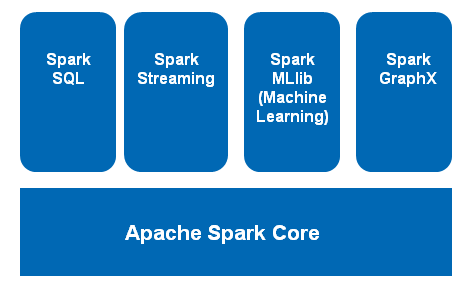
\includegraphics[scale=1.00]{Spark_ecosystem}
	\caption{Apache Spark Ecosystem \cite{spark:website}}
	\label{fig:ecosystem}
\end{figure}


\subsubsection{Spark Core}
\label{Spark Core}
Spark core is the heart to the APIs that exemplify Resilient Distributed Datasets (RDDs). The RDD API provides a programming interface for substantial scale data processing. These APIs can be programmed in Scala, Java, Python, and R. Besides, Spark Core is responsible for shuffling and scheduling of tasks, memory management between nodes in a cluster. Furthermore, libraries on top of the Spark Core handle diverse workloads. By optimizing the Spark Core, these libraries can be optimized.

\par  Resilient Distributed Datasets (RDD) are primarily responsible for data abstraction in Spark Core and are discussed in detail in the succeeding section. 

\textbf{Resilient Distributed Datasets}
\par Resilient Distributed Dataset (RDD) is a large set of immutable objects that are distributed parallel across nodes in a cluster \cite{Zaharia2012}. Spark offers RDDs, Accumulators, and broadcast variables as major data abstractions to its users to program clusters and two shared variables which are of restricted type \cite{zaharia2010spark}. The RDD is constructed with the assistance from Direct Acyclic Graph (DAG) which is a tree lineage. This lineage helps RDDs evade from data replication by keeping track of its transformations. As a result, RDDs are fault tolerant and they benefit from re-computation of data when one of its partitions is lost due to failure \cite{salloum2016big}.

\par RDDs can be created in Spark by two following ways \cite{karau2015learning,spark:website}:
\begin{enumerate}
\item By accessing data from external sources
\item By caching or persisting from already available RDDs
\end{enumerate}


\begin{figure}[htbp]
	\centering
		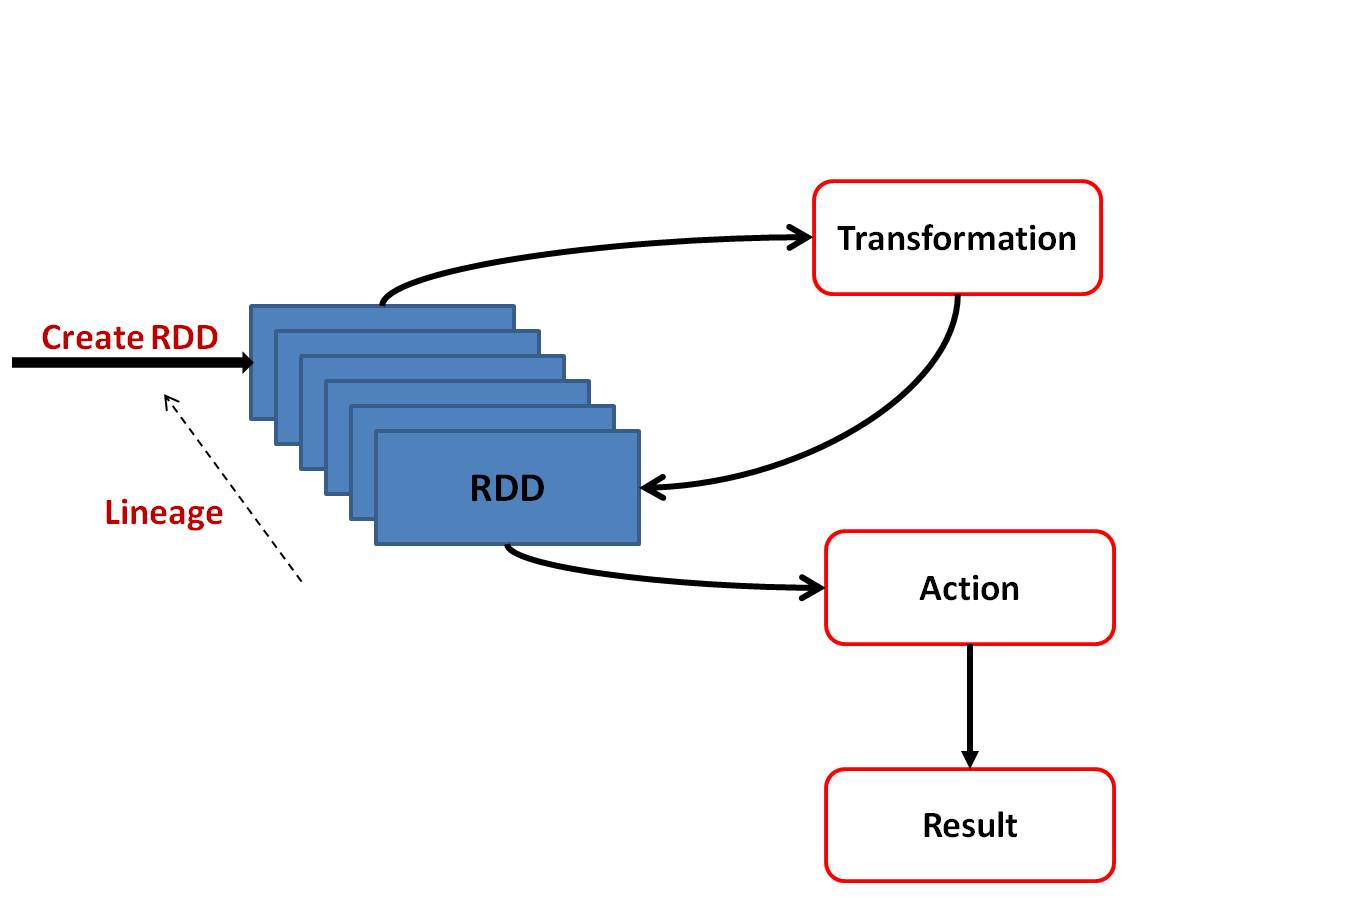
\includegraphics[scale=0.60]{RDD}
	\caption{Workflow of RDDs}
	\label{fig:RDDs workflow}
\end{figure}

\par As shown in \ref{fig:RDDs workflow}, there are mainly two types of operations namely Transformations and Actions that can be performed on RDDs \cite{zaharia2010spark,spark:website,karau2015learning}. 

\textit{Transformations:} From existing RDDs, a new transformed RDD is created using this operation. When a transformation operations are applied on RDDs, RDDs do not transform immediately until an action is called upon them. But instead, Spark remembers the metadata of transformations to be applied. Hence in Spark, these operations are termed as lazy evaluations. A bunch of these transformations operate element-wise (one element at a time) but not in every case \cite{karau2015learning}.

\par Part of the transformation operators usually used in Spark includes \cite{spark:website}:

\begin{itemize}
\item \textit{filter():} This operator is used when required to return selected elements from the previous dataframe through a function m.
\item \textit{map():} This operator returns a distinct dataframe by passing the function m to each element in the dataset.
\item \par\textit{join():} This operator is used to combine two dataframes with a join condition and returns a new dataframe. 
\item \textit{repartition():} This operator is used to randomly reshuffle the data partitions either to increased partitions by creating or fewer partitions by deleting across all the nodes in a cluster.
\end{itemize}

\textit{Actions:} After applying action operator on the RDDs, the resulting transformation returns the values to the driver program \cite{spark:website}.
\newline
\par Some member operators belong to this type include \cite{spark:website}: 

\begin{itemize}
\item \textit{collect():} Returns entire elements of a dataframe in the form of array to the driver program.
\item \textit{count():} This operator counts the total number of elements available in the dataframe.
\item \textit{take(m):} This operator returns the first m elements from the dataframe.
\item \textit{first():} This operator returns the first element in the dataframe.
\item \textit{reduce():} This operator merges elements in the dataframe with specified function m.
\end{itemize}


\textbf{Broadcast Variables} 
\par As discussed earlier in spark, Broadcast Variables comes under the hood of Shared Variables which are used for specific purpose. As a rule, the functions like map, reduce are executed by copying every variable associated with the function on all nodes in a cluster. But any update on these variables from any node will not be transmitted back to the driver program \cite{spark:website}.

\par Instead of copying all the variables associated with the task, Broadcast variables are cached to all nodes in a cluster irrespective of their association. Use of Broadcast variables is advantageous when there is a need for the huge volume of input dataset to be cached on all nodes. With broadcast algorithms, Spark can efficiently distribute the broadcast variables across all the nodes and also minimize the communication between nodes \cite{spark:website}.

\subsubsection{Spark SQL}

\par Spark SQL is another rich library built on top of Spark Core. Spark SQL is developed to perform relational database related query operations on RDDs but limited to structured and semi-structured data. Any data is said to be structured if every record in a dataset was defined with a schema. Similarly, if the schema can be defined explicitly then the data is said to be semi-structured. Spark supports to read data from formats like Hive tables, JSON, Parquet. Using Spark SQL on big data, all the relational SQL queries can be performed in parallel \cite{spark:website}. 

\par The fundamental aspect which makes Spark SQL differ from Spark RDD API is the interface offered by Spark SQL. This interface provides additional information related to the data structure alongside computations to Spark. With this additional information, Spark SQL can perform further optimizations.


\par Moreover, Spark SQL is now capable of integrating SQL queries and procedural code in one single application. Thus, with this integration Spark can perform complex analytics. For instance, processing of machine learning algorithms and graph algorithms on diverse big data applications. Spark SQL achieved this intermix by two models namely DataFrame API and optimizer titled Catalyst \cite{armbrust2015spark}.

\par In the consecutive sections, DataFrames are discussed in detail.

\textbf{DataFrames}

\begin{figure}[htbp]
	\centering
		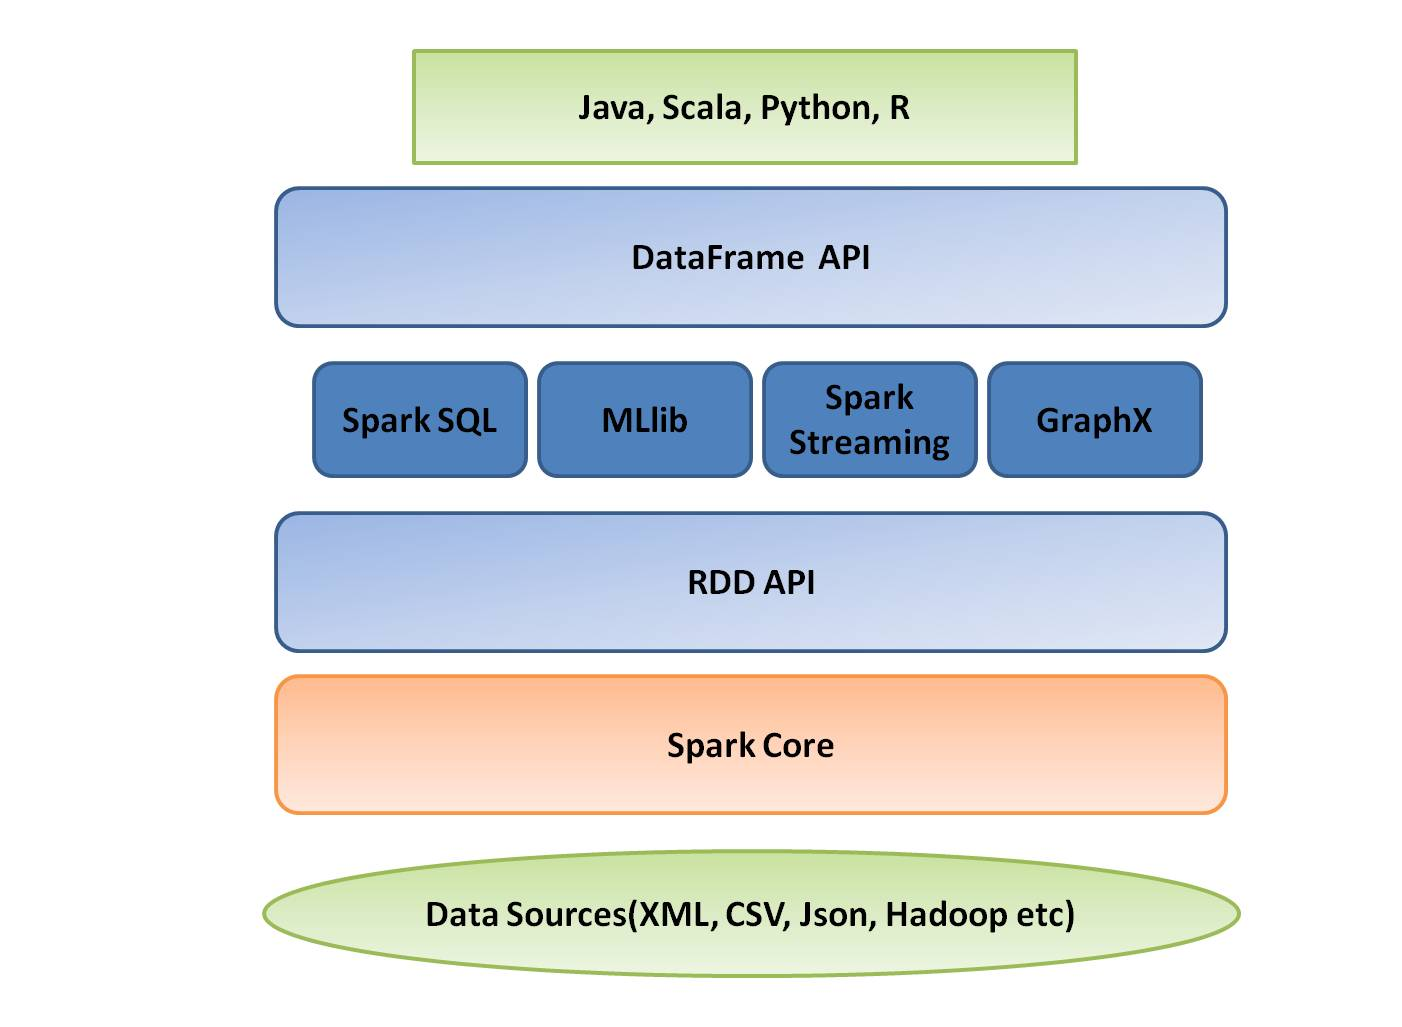
\includegraphics[scale=0.60]{DataFrames_API}
	\caption{DataFrame API in Spark Ecosystem }
	\label{fig: DataFrame API}
\end{figure}

\par DataFrames are generally known abstractions of tables in Python and R. For Structured Data and semi-structured data, the DataFrame API provides a high level abstraction of the Spark SQL. Similar to RDDs, DataFrames are also large sets of distributed data collection but with organized named columns as well as maintain a record of their schema for increased optimizations. Scala, R, Python, and Java support DataFrame API and illustrated in \ref{fig: DataFrame API}. DataFrames can be constructed with multiple sources ranging from existing RDDs to external databases. In Python, the DataFrame on a conceptual level is identical to a relational database table \cite{spark:website}.


\begin{figure}[htbp]
	\centering
		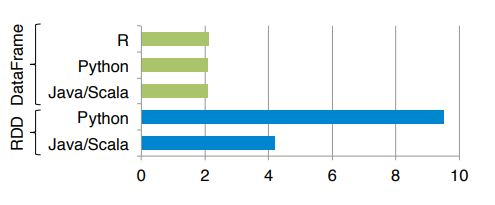
\includegraphics[scale=1.00]{RDD_vs_Dataframe}
	\caption{Difference in Execution time (Seconds) taken by RDD API and DataFrame API for a aggregation query using distinct programming languages \cite{armbrust2015scaling} }
	\label{fig: RDDvsDataFrame}
\end{figure}

\par The compelling feature of the DataFrame is storage of data in a columnar fashion which is much more consistent than Java/Python objects. As shown in \ref{fig: RDDvsDataFrame}, DataFrames can compute multiple aggregations efficiently using a single SQL statement when compared to Spark functional API irrespective of the programming language \cite{armbrust2015spark}. Within Spark applications, DataFrame APIs provide functional integrations with Spark SQL to other libraries. As a result, DataFrames are now prime representations to Spark's ML Pipeline API, GraphX and GraphFrames \cite{karau2015learning}.

\par Antithetical to Spark APIs, DataFrames hold relational operations as domain-specific language (DSL) expressions which then translate to abstract syntax trees (AST) and send to Catalyst optimizer to ensure optimization. This functionality enabled DataFrames to compute efficiently and conveniently than RDD API. Furthermore,  DataFrames in Spark is lazily evaluated which means there will be no execution of the logical plan until the user calls an action. The logical plan is stored as an individual DataFrame object for computations on dataset \cite{armbrust2015spark}. Apart from these, DataFrames not only restricted to use of its built-in functions but also supports User Defined Functions (UDFs) in which user can define own functionality to their applications.

\par The DataFrame API provides a variety of operations that can be performed on a DataFrame. Segment of these operators like alias(), count(), cache(), withColumn(), repartition() are used in our application and are described below \cite{spark:website}:

\textit{alias():} With this operator, a new DataFrame can be created by replicating the original DataFrame.

\textit{cache():} With the use of this operator, DataFrame will be cached to in-memory.

\textit{count():} Count operator counts the total number of rows that a DataFrame consists and returns the value.

\textit{repartition():} With this operator, a DataFrame can be equally partitioned into \textit{p} partitions.

\textit{withColumn():} Either by creating a new column or replacing a column can be performed to the existing DataFrame by use of this operator. For instance, if a DataFrame has two columns (\textit{Col a, Col b}) then a third column (\textit{Col c}) can be added to it by invoking this operator.

\subsubsection{Spark Machine Learning (MLlib)}

\par To process large scale datasets that require iterative algorithms in a distributed environment, Spark provides a high level machine learning API build on top of Spark Core as illustrated in \ref{fig:ecosystem}. As Spark benefits from in-memory computations, it makes convenient for iterative machine learning applications because any enhancements applied to Spark Core enhances the performance in upper-level libraries without explicit changes to the upper-level libraries. Hence improved enhancements in Spark MLlib with Spark's integration.

\begin{figure}[htbp]
	\centering
		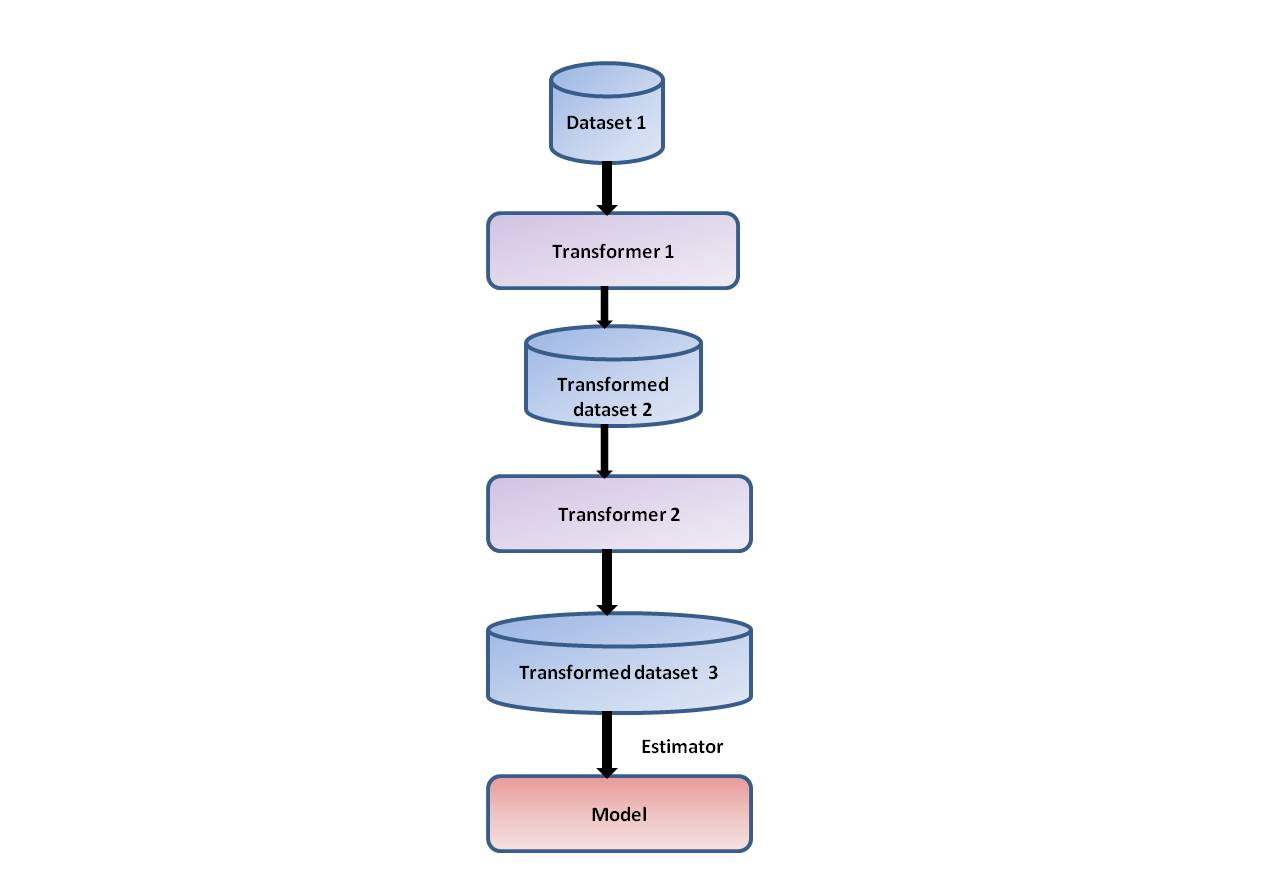
\includegraphics[scale=0.75]{pipeline}
	\caption{An example machine learning workflow with transformers and estimators}
	\label{fig: pipeline}
\end{figure}

\par Machine learning in Spark is divided into mllib and ml packages. The package mllib is built on top of RDDs whereas package ml is built on top of DataFrames. According to \cite{spark:website}, Spark now uses DataFrame-based API as prime machine learning API as the DataFrames are advantageous in many scenarios than RDDs including its optimized computations, simplified data integration to Spark SQL. The conversion of DataFrame to RDD and vice-versa can be applied to all algorithms of the Spark's Mllib by swapping conveniently from ml to mllib.


\par Spark's machine learning library comes with a variety of machine learning techniques include  Clustering, Transformers, Extractors, Classification, Clustering, Dimensionality Reduction. Like Spark Core, Spark Mllib also supports Scala, Java and Python programming languages to develop scalable machine learning algorithms. Additionally, it also supports a wide range of statistics, evaluation methods and linear algebra that are generally required for general machine learning applications for purpose of analytics \cite{meng2016mllib}.



\par Generally, many of the machine learning applications process data in sequential stages that involve preprocessing to validation stages which are commonly referred to a pipeline. Spark MLlib provides the pipeline functionality through ml API to construct efficient data workflows in a simplified manner. Each stage in the ml pipeline contains Transformers and Estimators. Transformer receives the input dataset, performs a transformation technique that is chosen and the output of the transformed data is fed into next stages of ml pipeline. Usually, these transformers in machine learning are used for feature extractions from input dataset. Likewise, an estimator is used for producing a model with the transformed data. An estimator is always followed by a transformer and is illustrated in \ref{fig: pipeline}. Pipelines are useful to configure any number of stages for a large scale machine learning applications \cite{website:databricks}. 

\par From \ref{fig: pipeline}, we can observe that the size of the dataset is increasing after it is fed into transformers. This is because when a transformer transforms data, a new column is generated as an output column for the transformation technique applied and then finally a model is produced by invoking the estimator.


\textbf{Vectors}

\par Under the mllib package, Spark represents two vector classes called Sparse Vectors and Dense Vectors for the purpose of vector related computation processing. Sparse Vectors stores only non-zero values to an array object where as Dense Vector stores all the values in an array of objects and can be used for mathematical calculations with other array objects. But, Spark allows Dense Vectors to store values as numpy floating object which translates to that even if an integer value is passed to the vector the resulting vector would be of type float. With the help of RDD transformations, these dense vectors can be distributed to all other RDDs as these objects are locally exist intrinsically \cite{website:densevectors} \cite{website:documentation}.



\subsubsection{Spark Streaming}

To process the huge amount of data in real-time, Spark Streaming library was developed as an extension to Spark Core API. A programming model called discretized streams or (DStreams) is the primary abstraction for Spark Streaming. The RDDs arranged in series represent DStreams. With a wide range of input streams namely Twitter, Kafka, Flume and etc DStreams can be created and then can be transformed to databases. Moreover, DStreams can also be created by other DStreams. Scala, Java and Python APIs are supported by Spark Streaming. Every RDD created by DStream contains the data with a specific time interval which can be referred as micro batching. With Spark Streaming, a streaming application that requires scalability, as well as fault tolerance as factors can be built \cite{spark:website}.

\subsubsection{Spark GraphX}
 For distributed environments, Spark offers GraphX library to process graph based data computations. 

As our application does not require Spark GraphX and Spark Streaming, We have briefly discussed them.

\subsubsection{Management of Clusters}
\label{section: management of clusters}
Spark requires cluster managers to access data from external sources encompassing Cassandra, HBase, HDFS \cite{Jonnalagadda2016}. Spark Core is built on top of cluster managers to facilitate this purpose. The job of the cluster manager is to allocate and supervise available cluster resources between spark applications. Spark not only runs on its standalone cluster manager but also integrates with distinct cluster managers accommodating Hadoop YARN, Apache Mesos, and Amazon EC2 \cite{karau2015learning}.


\par Spark application can be submitted by either local mode or cluster mode. To process the huge voluminous data, cluster mode is used. On the other hand, a local mode is used for the purpose of testing the application. The cluster mode functions in master/slave architecture where the slaves are connected in a distributed environment. The slaves are also called as workers. When an application is launched in cluster mode, then the master node divides the program execution into smaller chunks and are distributed across the workers.

\section{Related Work}
\label{section: Related work}
In this section, previously carried out implementations in the area of document matching as well as Latent Dirichlet Allocation are discussed. Various concepts exist to improve the execution time in the field of LDA algorithms with parallel computational processing.  \ref{subsection: mpi based} and \ref{subsection: Mapreduce based} provides information on such implementations which focuses primarily on improving the LDA algorithms for parallel environments. Only few relevant concepts that we think mostly related to this thesis are discussed although many implementations exist.


\subsection{MPI Based Implementation}
\label{subsection: mpi based}
MPI abbreviates to Message Passing Interface. MPI uses message passing programming model. MPI benefit from Universality, Expressivity, and Ease of debugging. MPI is most widely used programming model to implement algorithms using parallel processing. MPI is not a language but a library provided to implement parallel computing applications \cite{gropp1999using}. The paper \cite{wang2009plda} discuss the parallel implementation of the Latent Dirichlet Allocation (LDA) using MPI programming model. The implementation uses AllReduce algorithm in assistance with the MPI. The major focus of the implementation was to parallelize the process of topic assignment of the documents in the huge collection thereby achieving the scalability. Finally, the authors measured the speed up and execution time of the implementation. The authors also made available the source code of MPI implementation under Apache open source License.

\subsection{MapReduce Based Implementation}
\label{subsection: Mapreduce based}

In the same paper \cite{wang2009plda}, the authors discusses the implementation of LDA using MapReduce programming model. In \ref{section: Mapreduce}, the core concepts regarding the MapReduce programming model along with its advantages and limitations are discussed in detail. The implementation processes the huge volume of data by dividing and distributing them across multiple workers in a cluster. As discussed in \ref{section: Mapreduce}, the MapReduce programming model consists of two stages namely map and reduce. The authors defined the map phase as sampling phase where the topic assignment of the documents using Gibbs algorithm takes place. Then, the reduce phase receives these topic assignments and update the model. The implemented application is then measured for Speedup and execution time. The two datasets namely Wikipedia and Forum dataset are used for evaluating the speedup performance. A comparison was made between the MPI based and MapReduce based implementations where the implementation based on the MPI overrules the MapReduce based implementations and the reasons are discussed.


\par The work in  \cite{elsayed2008pairwise} discusses the problems associated with the computations of pairwise document matching based on their similarity within a set of documents in huge volume. The author presented an implementation using MapReduce programming model as a solution to the above addressed problem. The chief purpose of the paper focuses on processing the huge set of documents by representing them as a bag of words irrespective of the order along with their term weights. The term weights provide information of the term importance in any document. The implementation processes indexing of documents in Map phase and computes pairwise similarity in reduce phase. The implementation was evaluated on cluster consists of 20 machines and calculated the runtime performance. For evaluation, the AQUAINT-2 dataset is used. 

%- Allgemeine Wissensgrundlagen des Fachgebiets
%- Spezielle Grundlagen, die für das Verständnis erforderlich sind
%- Rahmenbedingungen für die Arbeit
%- Ausführungen zum Stand des Wissens / der Technik
%Als Leitprinzip gilt: Nur Informationen erwähnen, die
%- später benötigt werden,
%- notwendig sind, um die Arbeit oder ihre Motivation zu verstehen
%Das heißt insbesondere,
%- keine Inhalte aus Lehrbüchern, außer
%- diese werden benötigt, um Problemstellung oder Lösungsweg zu definieren.

\chapter{Concept of Spark based Semantic Document Matching}
\label{concept}

In this Chapter, We discuss the motivation involved in the design and implementation of the document matching application using Apache Spark. In \ref{section: Idea}, we discuss the idea of our application. In \ref{section: workflow of spark based document matching}, We discuss the stages involved in implementation procedure of Document matching application.

\section{Overview}
\label{section: Idea}
As discussed earlier in \ref{background}, matching the similarity between two documents based on their semantics using TF-IDF model is not reliable. The TF-IDF techniques are mostly dependent on word occurrences in any document. But, Latent Dirichlet Allocation (LDA) represents any given document in terms of topic distribution by discovering the latent topics as discussed in \ref{section: lda}. 

\par The latent topics found by LDA translates to the contextual representation of a document. The context of the document speaks about how a document is structured. If we have the structure of the documents in terms of topic distribution then why should not the documents be compared?  This question has motivated us to design and implement the document matching application using LDA technique.

\par On the other side, we aimed to process the huge collection of documents. In recent times, MapReduce has been widely used programming model. But MapReduce has some performance limitations when compared to Apache Spark primarily in the area of iterative algorithms and are discussed in \ref{section: Mapreduce}. Since our motivation also includes in reducing the execution time of the application, we have used the Apache Spark as our parallel processing framework. The processing of in-memory computations, support for iterative algorithms are some of the advantages of Apache Spark and additional information is available in \ref{section: apache spark}.

\par Our objective was to increase the efficiency of our application and also present the potential of the Apache Spark framework. We did not made any modifications or improvements to the LDA algorithm but focused on finding a way to reduce the execution time.

\section{Workflow of Spark based Document Matching}
\label{section: workflow of spark based document matching}

As we have discussed our idea behind document matching using LDA. We now discuss the working model of our document matching application. The implementation of our application consists of 8 stages starting from loading of data to evaluation stage. The working process of our application using Apache Spark components is illustrated in \ref{fig: Implementation_process}.
\begin{figure}[htbp]
	\centering
		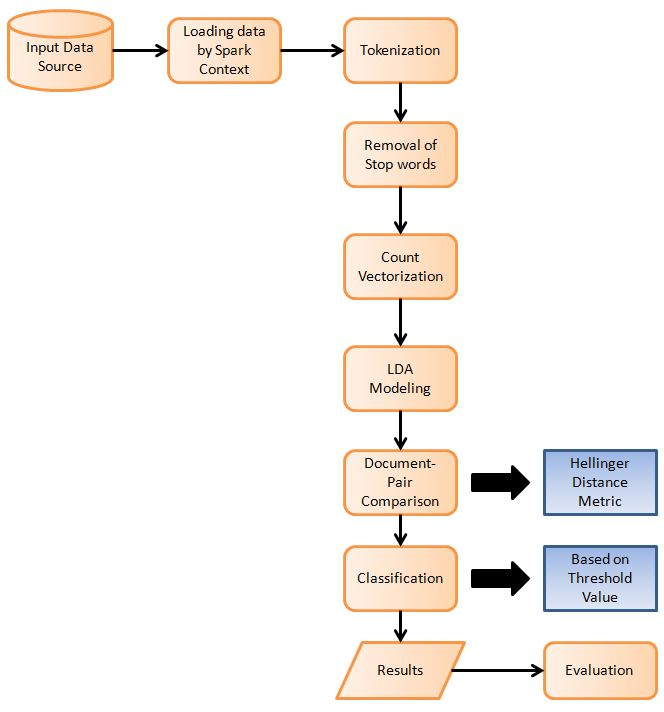
\includegraphics[scale=0.90]{implementation_process}
	\caption{Implementation procedure for Document Matching Application}
	\label{fig: Implementation_process}
\end{figure}

\newpage
\par From \ref{fig: Implementation_process}, the initial stage of our implementation starts by loading data from the external sources. It is a corpus in our case. The data will be loaded as a DataFrame with the help of Spark SQL.Each row of the DataFrame represents one document. The data in DataFrame is then sent as input to the tokenizer which extracts features from the document. In Stop words removal stage, further cleaning of the data such as removal of English stop words that do not contribute to the term importance is performed on the output of the tokenizer stage. In Count Vectorizer stage, every unique term is mapped to a unique ID and converts the documents to a sparse vectors representation. It is now time for topic modeling using LDA technique in LDA modeling stage. The total documents are compared with each other and an additional column containing match score is added to the DataFrame in the Document Pair Comparison Stage. Using the predefined threshold value, the document pairs are classified as matches and non-matches in the classification stage. The document pairs classified are then stored as a DataFrame. In the evaluation stage, the classified pairs are evaluated as true positives, false positives, true negatives and false negatives. 

\par Using Apache Spark framework, it is possible to execute each stage of our application individually by storing each stage result and then feeding as input to the future stage. Alternatively, all the stages can be executed as a chain of processes without writing intermediate results to the disk. The requirements, the details of our Spark based Document Matching implementation and the transformations of data at every stage are discussed in \ref{implementation}.



\chapter{Implementation of Spark based Semantic Document Matching}
\label{implementation}

In this chapter, we discuss the details involved in the implementation of the spark based Semantic Document Matching application. In \ref{section: implementation preferences}, we discuss in nutshell about the software and hardware preferences, dependency plug-ins and about the libraries from external sources that we used in our application. From \ref{section: loading data}, we discuss about how the implementations performed in detail and the example results for enhanced perspective.


\section{Implementation Preferences}
\label{section: implementation preferences}
In this section, we discuss the details of the implementation environment and the requirements which we used for our application development in various stages.

\subsection{Software Preferences}
We have used Python 3 as our programming language as it supports interactive shell, lambda expressions, and DataFrames. Though Python based implementation takes more time than Java and Scala based implementations with RDD APIs, it do not affect the performance of the DataFrame API. To carry out development on Ubuntu operating system, We used a virtual box environment called VMware and the following software are installed in the virtual environment:

\begin{itemize}
\item Python 3
\item PySpark 2.2
\item Jupyter notebook
\end{itemize}




\subsection{Plugin Preferences}
We have used Numpy and Scipy libraries \cite{website:numpy} for faster vector computations. To parse the extensible Markup Language (XML) file, we have used databricks XML data source library \cite{website:xmlspark}. It is an official API for the spark to read XML files by databricks. We also used Py4j library which connects the bridge between Python interpreter and the Java virtual machine \cite{website:py4j}. For parsing of XML documents in a non-parallel environment, a library available as python extension called minidom is used \cite{website:minidom}.


\section{Loading Data}
\label{section: loading data}
As illustrated in \ref{fig: Implementation_process}, the initial process of our application starts with the loading of data. The data we have chosen is in XML format and the glimpse of a single file can be seen in \ref{fig:reutersdoc}. Using databricks XML data source API and Spark SQL, the data is loaded into a DataFrame with a manually specified schema. For the process of document matching, we require each document id and associate paragraphs. Hence on performing SQL select operation on the input DataFrame, we get the \ref{fig: loadingdata1} as the initial DataFrame with two columns namely DocId and text where DocId is the identity of each document and text holds the paragraphs. Once the data is loaded into a DataFrame, with the use of show(), describe(), printSchema() methods the data can be analyzed. By default, the show method returns the first 20 rows of the DataFrame.
From \ref{fig: loadingdata1}, we can observe that the data in text column is raw which also contains special characters. Hence the next stage would be cleansing of the data. The code snippet for this stage is illustrated in \ref{lst:parsing and loading data}

\begin{lstlisting}[style=Java,float=htb,caption={Python code for parsing and loading of data into a DataFrame},label={lst:parsing and loading data}]
xmlDf = spark.read.format('com.databricks.spark.xml').\
	options(rowTag='newsitem').load('<fileDirectory>',schema= custom)
df_first= xmlDf.select(col("_itemid").alias("DocId"),'text')
\end{lstlisting}

\begin{figure}[tbp]
	\centering
		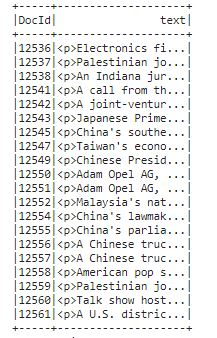
\includegraphics[scale=1.0]{loadingdata1}
	\caption{An output from loading data stage}
	\label{fig: loadingdata1}
\end{figure}

\section{Tokenization}
As discussed in the \ref{background}, the process of splitting a sentence or paragraph into individual words is referred as tokenization. ML package in Spark provides a powerful tokenizer API with which the process of the  tokenization can be performed. The tokenizer API is a transform function provided by the spark's ML library that transforms a DataFrame from one form to another form. The tokenizer API also supports the removal of special characters using regular expressions. Using regular expressions function, We have described the function to remove all the special characters, the numerical characters and convert all the words containing upper case to lower case. we have also described the minimum length of a character to be tokenized as 2 as a pre-requisite in order to retrieve the most meaningful words from the input dataset. The tokenizer API takes the text column as the input and returns an array of words in the new column. As shown in \ref{lst:tokenization}, with the tokenizer API, we can name the new column and we have named the new column as Words and is illustrated in \ref{fig: tokenization_output}. Using transform() operation, the tokenization is applied on the input DataFrame.

\begin{lstlisting}[style=Java,float=htb,caption={Python code for tokenization},label={lst:tokenization}]
tokens = RegexTokenizer(minTokenLength=2,inputCol='text',\
		 outputCol='Words', pattern="[^a-z]+") 
Tokenized = tokens.transform(df_first)
\end{lstlisting}

\begin{figure}[htbp]
	\centering
		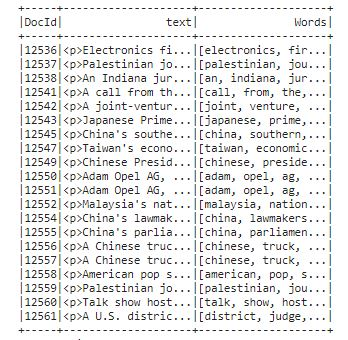
\includegraphics[scale=1.20]{tokenization_output}
	\caption{An output dataframe after tokenization stage }
	\label{fig: tokenization_output}
\end{figure}

\section{StopWords Removal}
As our input data is a huge collection of news articles, they often contain stop words in frequent. It is essential to clean those stop words in order to get meaningful terms. Spark's ML library provides the StopWords Remover function. It also comes under the transform function. The function takes an array of strings as input, applies the function and returns a new DataFrame with the addition of output column. The output DataFrame from this step is illustrated in \ref{fig: stopwords_output}.  The function is applied using transform() operation on the output DataFrame from the tokenization stage. The code snippet for this stage is shown in \ref{lst:stopwords}.

\begin{lstlisting}[style=Java,float=htb,caption={Python code for removal of stop words},label={lst:stopwords}]
Tokens_filtered = StopWordsRemover(inputCol='Words',\
				  outputCol='filtered_words')
Tokenized_filtered = Tokens_filtered.transform(Tokenized)
\end{lstlisting}

\begin{figure}[htbp]
	\centering
		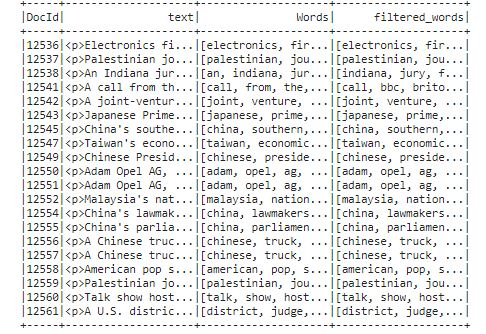
\includegraphics[scale=1.20]{stopwords_output}
	\caption{An output dataframe after cleaning of stop words }
	\label{fig: stopwords_output}
\end{figure}

\section{Count Vectorizer}
As discussed earlier in \ref{section: countvectorizer}, with the help of count vectorizer, any document can be converted to a sparse vector representation. Spark provides this functionality under the hood of extractors in the ML package. In order to convert a document into a sparse vectors, the function requires fit() and transform() operations as shown in \ref{lst:count vectorizer}. Firstly, on applying fit() operation the count Vectorizer builds a model by mapping the unique words to unique IDs that are extracted from the filtered words column. When transform() operation is applied, the count vectorizer transforms the documents representing an array of words to a sparse vector with the help of a dictionary. From \ref{fig: cv_output}, we can observe the DataFrame containing various stage of transformations of a document starting from loading of raw data to sparse vector representation of a document. 

\begin{lstlisting}[style=Java,float=htb,caption={Python code to perform count vectorization},label={lst:count vectorizer}]
cv = CountVectorizer(inputCol="filtered_words", outputCol="features")
cv_model = cv.fit(Tokenized_filtered)     
result = cv_model.transform(Tokenized_filtered)
result1 = result.select('DocId','features')
\end{lstlisting}

\par As discussed earlier about the vector representation of a document, we can observe from the features column in \ref{fig: cv_output} for a given example input, the total number of unique terms found by the count vectorizer model is 9844 which can also be referred as vocabulary size.

\begin{figure}[htbp]
	\centering
		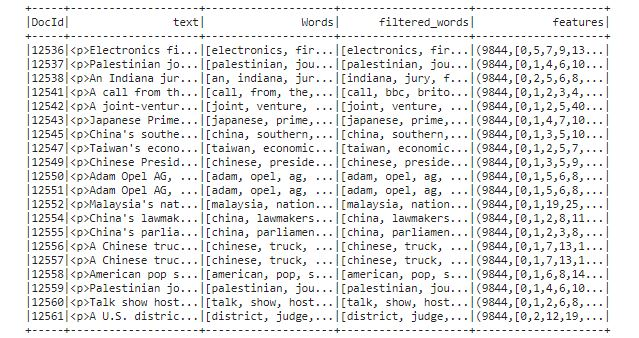
\includegraphics[scale=0.90]{cv_output}
	\caption{An output dataframe after performing count vectorization on input words }
	\label{fig: cv_output}
\end{figure}


\begin{figure}[htbp]
	\centering
		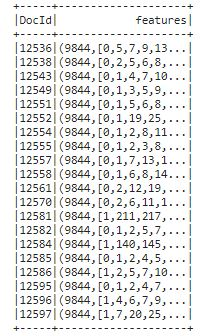
\includegraphics[scale=1.00]{cv1_output}
	\caption{An output dataframe after performing SQL Query }
	\label{fig: cv1_output}
\end{figure}

\par Additionally, the count Vectorizer model provides various parameters for tuning the model while creation. By default, the count vectorizer function selects the terms whose frequency of appearance is at least two times. But, we have set the value to 1 as we need each and every word that constituting to the document. On performing Spark SQL select operations on the DataFrame as in \ref{fig: cv_output}, we have only taken two columns and can be seen in \ref{fig: cv1_output} since the next stage only relays on feature column and DocId column. By reducing the DataFrame size, we can reduce the load on in-memory computations there by increasing the performance of the application.  


\section{Latent Dirichlet Allocation}
Recollecting from \ref{section: lda}, LDA approach is used for two reasons. The prime reason is to represent the document in terms of topic distribution and the other is to reduce the dimensionality of the vector representation achieved from the previous stage.

\begin{lstlisting}[style=Java,float=htb,caption={Python code to perform LDA Topic Modeling },label={lst:LDA}]
lda = LDA(k=90,maxIter=20,optimizer = "em")       
model = lda.fit(result1)
lda_df = model.transform(result1)
\end{lstlisting}


\par We have used LDA API under the Spark's ML package. From the \ref{lst:LDA}, the number of topics (k) that a document to be presented has to be manually specified. Hence, we have set the topics(K) to 90. Similarly, the number of iterations also has to be manually specified. The iterations represent the times an Estimation-Maximization (EM) algorithm has to infer the topics. At first iteration, the EM algorithm randomly assigns the words to every topic. From the second iteration, the M-step updates the parameters by learning the latent topics discovered from the previous iteration and the word assignment to topics based on the present parameters is performed again at each iteration. Since our focus was not to calculate the convergence but the runtime, we have set the iterations to 20. LDA also requires fit() and transform() operations to build the topic distribution. 

\begin{figure}[htbp]
	\centering
		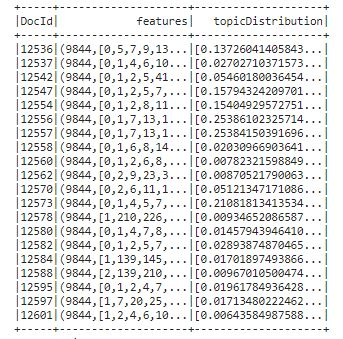
\includegraphics[scale=1.20]{lda_output}
	\caption{An output dataframe consisting of topic distribution after LDA modeling on the input dataset }
	\label{fig: lda_output}
\end{figure}

\par When fit() operation is applied on DataFrame from the previous stage as in \ref{fig: cv1_output}, LDA starts constructing the document topic matrix from a sparse vector. At this state, the entire input dataset is divided to all worker nodes in a cluster. The worker nodes construct topic distributions locally with the available data and send back to the driver using broadcast variables resulting in a huge combined matrix. Now, when the  transform() operation is applied, the DataFrame transforms to the other consisting of an additional column named topicDistribution. The output DataFrame is illustrated in \ref{fig: lda_output}. As we set the number of topics to 90, every document is represented by a vector of 90 dimensions and are in dense vector representation.  Since the LDA representation of the document is a probabilistic distribution, the summation of all topic values results to 1 for every document.


\section{Document Pair Comparison}
\label{implement: Document Pair Comparison}
In this stage, we perform a comparison of each document to every other document in the entire corpus. Using the Spark SQL, a self-join is performed on the Same DataFrame from the previous stage by aliasing the column names and is illustrated in \ref{fig: comparison}. Hence, this stage in the Document matching process consumes most of the time for performing the computations as the process requires a total of  \(O(n^2)\) computations.

\begin{figure}[htbp]
	\centering
		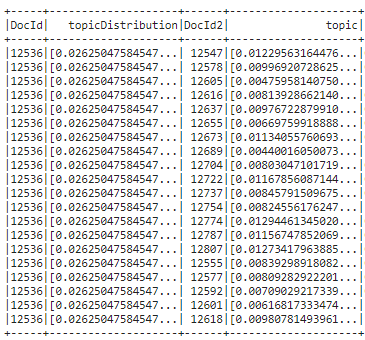
\includegraphics[scale=1.20]{comparison}
	\caption{An output dataframe after performing self join operation }
	\label{fig: comparison}
\end{figure}



For example, let us consider three documents namely Document 1, Document 2, and Document 3 present in a DataFrame. A total of 6 combinations results when a self-join is applied on the DataFrame and is illustrated in \ref{tab:combinations}. 


\begin{table}[htbp]
	\centering
		\begin{tabular}{cc}\toprule
		DocId	& DocId2\\\midrule
		1 & 2\\\addlinespace 
		1 & 3\\\addlinespace
		2 & 1\\\addlinespace
        2 & 3\\\addlinespace
        3 & 1\\\addlinespace
		3 & 2 \\\bottomrule
		\end{tabular}
	\caption{An example of document combinations}
	\label{tab:combinations}
\end{table}

\begin{equation}\label{formula: hellinger on two documents}
Hellinger(1,2) == Hellinger(2,1)
\end{equation}

But from \ref{formula: hellinger on two documents}, we can observe that the Hellinger metric assures from the symmetric property which translates to the result obtained by the product of any two documents are same irrespective of the order they appear. Hence, we have passed the \ref{formula: pair condition} as join condition in order to decrease the number of computations required in calculating the total document pairs. By passing this condition, we can eliminate computations of the document pairs that are symmetric to already computed pairs. For example, by applying \ref{formula: pair condition} the total computations in \ref{tab:combinations} can be reduced to 3 which translates to speed up of the computation process by a percentage of 50. The code listing is illustrated in \ref{lst:pairwise}.

\begin{equation}\label{formula: pair condition}
DocId < DocId2
\end{equation}

\begin{lstlisting}[style=Java,float=htb,caption={Python code to perform Document Pair Comparison },label={lst:pairwise}]
similarity_df = final_df.join(final_df.alias("copy_df").\
     	select(col("DocId").alias("DocId2"),col("topicDistribution").\
     	alias("topic")),col("DocId") < col("DocId2"), 'inner')
		.withColumn('Score',hellinger_udf(col('topicDistribution'),\
		col('topic')))
\end{lstlisting}


\par Using withColumn() operation, a new column named Score is added to the DataFrame as in \ref{fig: comparison1}. The result of calculating the distance between topic distribution of two documents is stored in the Score column. The score value represents the similarity between the two documents. The distance is calculated using Hellinger distance metric as already discussed in \ref{section: document pair comparison}. As Spark do not have the built-in Hellinger function, we have created a user defined function using Spark's udf() functionality.  

\begin{figure}[htbp]
	\centering
		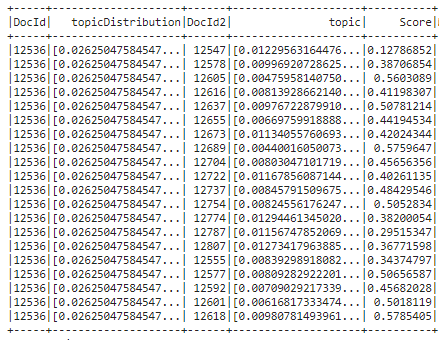
\includegraphics[scale=1.20]{comparison1}
	\caption{An output dataframe from Document Pair Comparison Stage }
	\label{fig: comparison1}
\end{figure}


\section{Classification}

In this stage, every document pair is classified as either match or non-match based on their obtained similarity score. A user defined function holding a threshold condition is manually specified to classify the document pairs using udf(). The condition for classification is shown in \ref{formula: threshold condition} and \ref{formula: threshold condition1} respectively where 1 represents that the two documents are semantically similar and 0 represents the documents are dissimilar.

\begin{equation}\label{formula: threshold condition}
\textit{Score}   >  \textit{threshold-value}  \Rightarrow Match = 0
\end{equation}
\begin{equation}\label{formula: threshold condition1}
\textit{Score}  \leq  \textit{threshold-value}  \Rightarrow Match = 1
\end{equation}


\par As shown in \ref{lst:classification}, using withColumn() a new column  named Match\char`_result is appended to the DataFrame from previous stage as shown in \ref{fig: classification}. The threshold function is performed on the column score and the obtained result is stored in the column Match\char`_result.

\begin{lstlisting}[style=Java,float=htb,caption={Python code to classify Documents along with threshold condition},label={lst:classification}]
def threshold(Score):
    if Score <= 0.2:
        return 1
    else:
        return 0
        
output_df = similarity_df.withColumn('Match_result',\
			threshold_udf(col('Score'))
\end{lstlisting}

\begin{figure}[htbp]
	\centering
		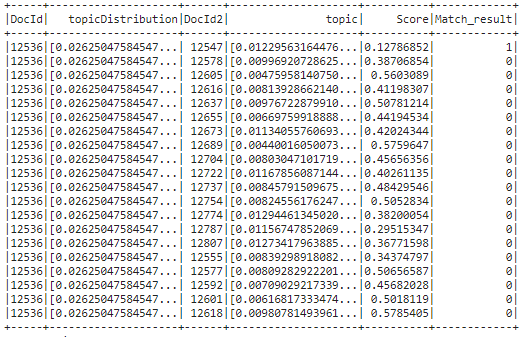
\includegraphics[scale=1.00]{Classification}
	\caption{An output dataframe from Classification stage }
	\label{fig: classification}
\end{figure}

\section{Evaluation}
\label{implement:evaluation}

The final stage in our implementation process is Evaluation. With the results obtained from the classification stage, evaluations are computed to calculate the speed-up, efficiency and effectiveness and are discussed in detail in \ref{evaluation}. 

\par To calculate the effectiveness of an implementation, the results obtained from our process need to be matched with the golden data. But as discussed in \ref{section: rcv1}, the corpus do not possess any ground truth information representing the similarity state of two documents but provides information of a document belongs to a topic. Hence we have implemented a workaround method to extract the topics from the metadata information available from each document. The glimpse of a document is presented in \ref{fig:reutersdoc}. The workaround method is implemented as a combination of parallel and a non-parallel environment i.e. with the combination of Python and Spark framework. The steps involved in workaround method is discussed below:


\subsection{Parsing XML}
\par Using minidom \cite{website:minidom} which is a Python extension library, each document is parsed to extract the topic information available under the metadata information. The data obtained is stored as a list of lists and is illustrated in \ref{lst:minidom}. Each list contains information of the document ID and list of topics, as a document can speak about different topics. Due to the complex structure of the input document, the extracted category information is obtained as a combination of regions and topics. Hence to increase the accuracy of the data, it is necessary to remove the regions from the topics.

\begin{lstlisting}[style=Java,float=htb,caption={Python Code to parse XML file to extract category using minidom library in non-parallel Environment},label={lst:minidom}]
from xml.dom import minidom
import os
directory = '<fileDirectory>'
finallist = []

for root,dirs,filenames in os.walk(directory):
        for file in filenames:
            #print(file)
            log = open(os.path.join(root,file),'r')
            doc = minidom.parse(os.path.join(root,file))
            idlist = doc.getElementsByTagName('newsitem')
            for id in idlist:
                value = id.getAttribute("itemid")
            codelist = doc.getElementsByTagName('code')
            words=[]
            for s in codelist:
                words.append(s.attributes['code'].value)
            finallist.append(value)
            finallist.append(words)

\end{lstlisting}

\newpage
\subsection{Removal of Regions}
\par As discussed in the earlier chapter, Spark provides many powerful tools for the purpose of pre-processing. One among them is stop words remover. To use the Spark's component, firstly the data is loaded into a DataFrame using a manually specified schema with createDataFrame() operation. Using the Reuters data file, a list consisting of all the region codes is generated as a stop words list . Using the stop words list, all the regions are removed and the DataFrame transformation is performed using transform(). The code for this step can be observed in \ref{lst:extract regions}.

\begin{lstlisting}[style=Java,float=htb,caption={Python Code for loading lists into DataFrame and filter regions},label={lst:extract regions}]
df_first = spark.createDataFrame([(x,y) for x,(y) in (zip(
            islice(finallist,0,len(finallist),2),
           islice(finallist,1,len(finallist),2)))],\
           ('DocID','Categories'))
Filter_regions = StopWordsRemover(inputCol='Categories',\
				 outputCol='Topics',stopWords=["list"])
\end{lstlisting}



\subsection{Pair Comparison} 

\begin{table}[htbp]
	\centering
		\begin{tabular}{cc}\toprule
		DocId	& Topics\\\midrule
		1 & Apple, Bat\\\addlinespace 
		2 & Bat, Cat, Dog\\\addlinespace
		3 & Apple \\\bottomrule
		\end{tabular}
	\caption{An example of document and topics}
	\label{tab:document topics}
\end{table}

This step is similar to the stage in the document matching process. In this step, we performed the comparison of each document with every other document. A self-join of the same DataFrame by aliasing the column names is performed. The similar join condition as in \ref{formula: pair condition} used in document pair comparison is used here also in order to obtain the exact document pairs. Using withColumn(), a new column is appended to the DataFrame named Intersect\char`_score. The score is generated as a true or false and is stored in the Intersect\char`_score column. Two documents are said to be true if any of the topics overlap between the two documents. It is false if there is no overlap in between two document topics. For example, let us consider three documents and the 4 topics. Each document is provided with topics that a document belongs to and is illustrated in \ref{tab:document topics}.


\begin{equation}\label{formula: pair condition for subset}
Topics(DocId) \subset Topics(DocId2) \Rightarrow True
\end{equation}
\begin{equation}\label{formula: pair condition for not subset}
Topics(DocId) \not\subset Topics(DocId2) \Rightarrow False
\end{equation}


Based on the \ref{formula: pair condition for subset} and \ref{formula: pair condition for not subset}, the \ref{tab:score generation} is generated.


\begin{table}[htbp]
	\centering
		\begin{tabular}{ccc}\toprule
		DocId	& DocId2 & Score\\\midrule
		1 & 2 & True\\\addlinespace 
		1 &  3 & True\\\addlinespace
        2 & 3 & False\\\bottomrule
		\end{tabular}
	\caption{A Table illustrating Score generation}
	\label{tab:score generation}
\end{table}

\subsection{Classification} 
Based on the Score obtained from the previous step, every document pair is classified as similar or dissimilar according to the \ref{formula: threshold condition for category} and \ref{formula: threshold condition1 for category} where 1 represents that a document pair contains the common topics between them and 0 represents that a document pair do not hold any common topics between them. A new column is appended to the previous stage DataFrame using withColumn() and the classification results obtained in this step are stored in this column.

\begin{equation}\label{formula: threshold condition for category}
\textit{Score}   \equiv  \textit{True}  \Rightarrow True\char`_match = 1
\end{equation}
\begin{equation}\label{formula: threshold condition1 for category}
\textit{Score}  \equiv  \textit{False}  \Rightarrow True\char`_match = 0
\end{equation}


\begin{figure}[htbp]
	\centering
		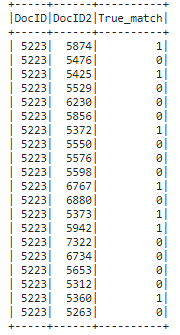
\includegraphics[scale=1.05]{category_extraction}
	\caption{An output dataframe obtained in the Category Extraction Process }
	\label{fig: category_extraction}
\end{figure}

\begin{lstlisting}[style=Java,float=htb,caption={Python Code for writing resulting DataFrame to parquet Format},label={lst:write parquet}]
Final.write.parquet('<FileLocation>')
\end{lstlisting}

\newpage
Finally as shown in \ref{lst:write parquet}, the resulting DataFrame obtained is written to the parquet file and is stored. The final DataFrame obtained after processing all the steps is shown in \ref{fig: category_extraction}. The DataFrame obtained from classification stage is compared to the DataFrame obtained in this process. By applying Spark DataFrame count() method on the resulting DataFrame, the number of True Positives, False Negatives, False Positives, and True Negatives are calculated with which measures like recall, precision and F-measure are calculated.







%In diesem Kapitel beschreiben Sie,
%- wie Sie versucht haben, Ihre Arbeit (z.B. Programm, Theorie, oder Algorithmus) zu verifizieren
%- Hierfür haben Sie bereits im Kapitel 3 Prognosen oder Qualitätskriterien aufgestellt, die Sie hier überprüfen
%Zu jeder zu überprüfenden Eigenschaft sollten Sie
%- ein geeignetes Experiment entwerfen, um diese Eigenschaft zu überprüfen
%- dieses Experiment beschreiben und durchführen
%- die Ergebnisse geeignet präsentieren und kommentieren

%wie lange dauert das schlussfolgern bei bestimmten veränderungen?
%wie lange für komplett unterschiedliche?



\ifgerman{\chapter{Evaluierung}}{\chapter{Evaluation}}
\label{evaluation}
We have performed various experiments in order to evaluate our Semantic Document Matching approach using Apache Spark. The details about the experimental procedure as well as the results obtained are discussed in this chapter. \ref{Section: Experimental Setup} provides information about the environmental setup used for the evaluation. In \ref{section: input dataset}, we discuss the details of the input dataset used for evaluations.

\section{Experimental Setup}
\label{Section: Experimental Setup}

In this section, We provide the details about the spark cluster as well as about the various size of the input data that are used for evaluations.

\subsection{Environment}

Evaluations are performed on a spark cluster that composes of 7 worker node and a master node. As mentioned earlier in \ref{section: management of clusters}, a spark program can be run either in a local mode or in a cluster mode. Cluster managers are required if a program needs to run in cluster mode and hence spark provides standalone cluster manager as well as supports other cluster managers includes Hadoop YARN and MESOS. We discuss about the software and hardware configurations of the cluster in the following sections.

\textbf{Hardware Configuration} 
\par As stated above, we have used a cluster consisting of 7 worker nodes and a master node. Each worker posses 4 processing cores and 6 Gigabytes of main memory. Though all the workers posses quad core processors but are in heterogeneous in nature. 

\textbf{Software Configuration}
\par We used Open VPN and SSH Secure shell to establish a connection to the cluster and also to upload the input dataset to the local file system. Every worker in the cluster has the following software installed on them:
\begin{itemize}
\item Ubuntu 64-bit operating system
\item PySpark 2.2.0
\item Python 2.7
\item Java 1.8
\end{itemize}


\subsection{Input Dataset}
\label{section: input dataset}
We have used Reuters corpus version1 (rcv1) to perform evaluations. The detailed discussions are pointed in \ref{section: rcv1}. Rcv1 totally contains 806791 documents organized into 365 folders. The total size of the corpus is 3.67 Gigabytes. To perform various evaluations, all the documents in the corpus are separated with varying sizes and are illustrated in \ref{tab:input dataset with various size}. 

\begin{table}[htbp]
	\centering
		\begin{tabular}{cc}\toprule
		Number of Documents in Input Dataset & Size in MB\\\midrule
		\(10^4\) & 29 \\\addlinespace 
		\(2*10^4\)  &  59 \\\addlinespace
        \(3*10^4\)  &  89 \\\addlinespace
        \(4*10^4\)  &  116 \\\addlinespace
        \(5*10^4\)  &  147 \\\addlinespace
        \(6*10^4\)  &  176 \\\addlinespace
        \(7*10^4\)  &  207 \\\addlinespace
        \(8*10^4\)  &  236 \\\addlinespace
        \(9*10^4\)  &  263 \\\addlinespace
        \(10^5\)  &  296 \\\bottomrule
		\end{tabular}
	\caption{A Table illustrating input dataset with various size}
	\label{tab:input dataset with various size}
\end{table}

\section{Experimental Procedure}
To evaluate the thesis and to optimize the implementation process, we have performed various experiments using the different sizes of the input dataset as shown in \ref{tab:input dataset with various size}. The cluster setup has also been varied according to the requirement of the experiment. In this section, We discuss the details of the experiments performed and how the procedure is carried out. 


\subsection{Experimental Procedure for Evaluation of Speed-up and Efficiency }
The primary focus of the thesis is to decrease the execution time of the Semantic Document Matching process in a parallel environment. To analyze the parallelism achieved by the implementation process, We have calculated the Speed-up and Efficiency. We have evaluated the approach with varying number of worker nodes ranging from 2 to 7 in the cluster and the memory usage of each worker node is set to 6 Gigabytes. To analyze the parallelism of the implementation process, we require a large voluminous input dataset. Hence we have evaluated this experiment with the input dataset consisting of \(10^5\) documents as shown in \ref{tab:input dataset with various size}.  

\par The evaluation is carried out by calculating the total execution time taken by the approach starting from the loading stage to the classification stage. We have not considered the evaluation stage for this experiment. The results obtained for the experiment are discussed in \ref{subsection: evaluating speed-up and efficiency}.

\subsection{Experimental Procedure for Evaluation of Threshold based Classification }

To analyze the parallelism achieved by the classification stage, we performed this experiment with varying amounts of input dataset using 7 worker nodes in the cluster. The varying amounts of input dataset are illustrated in \ref{tab:input dataset with various size}. The worker nodes are not varied in this experiment. With this experiment, the total runtime taken by the implementation process for classification stage is calculated and the results obtained are discussed in \ref{subsection: evaluating threshold}.


\subsection{Experimental Procedure for Effectiveness Evaluation}

The aim of this experiment is to evaluate the quality of the results obtained by the entire Semantic Document Matching process. As discussed earlier in \ref{section: rcv1}, the input dataset Reuters Corpus Version 1 (rcv1) do not possess any information on the ground truth describing the semantic similarity between two documents. Hence, we have designed a workaround method and the detailed discussion can be found in \ref{implement:evaluation}. The ground truth table was generated by implementing the workaround method for \(10^4\) documents and is used for this experiment. The quality measures like precision, recall, and F-measure are calculated. The obtained results are discussed in \ref{subsection: evaluating effectiveness}.


\section{Evaluation Results and Discussion}

In this section, we discuss the results obtained for the above discussed experiments.

\subsection{Evaluating Speed-up and Efficiency}
\label{subsection: evaluating speed-up and efficiency}

By varying the worker nodes of the cluster, We have evaluated the runtime, speedup, and efficiency of the Semantic Document Matching process. The runtime of the approach was calculated from starting of spark context till the classification stage. On one worker node, it took 55 minutes to process the \(10^5\) documents. It is then reduced to 18 minutes on an average when run on 4 worker nodes but again increased. When the application was run on 7 workers nodes of the cluster, the execution time was reduced to 14 minutes on an average. The execution time for varying number of worker nodes is illustrated in \ref{fig: result_runtime}. But on performing optimizations on the implementation process, we have succeeded in further reducing the execution time of the process and is illustrated in \ref{fig: result_improved_runtime}. The performed optimizations are discussed in \ref{section: Discussions}.

\begin{figure}[htbp]
	\centering
		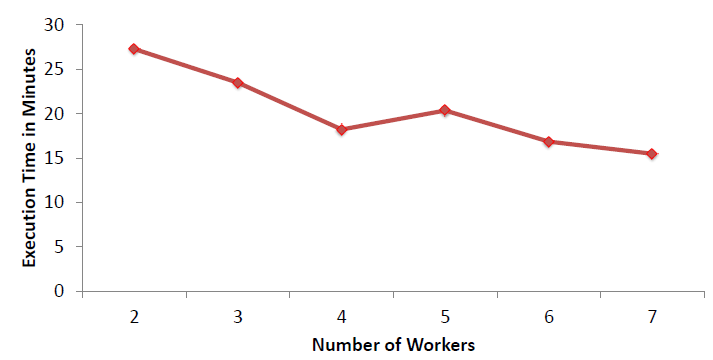
\includegraphics[scale=0.80]{runtime_result}
	\caption{Execution Time for processing \(10^5\) documents, Topics (K) = 90, Iterations = 20, Vocabulary Size = 137462, Total Document Pairs Classified =  4999950000}
	\label{fig: result_runtime}
\end{figure}

\begin{figure}[htbp]
	\centering
		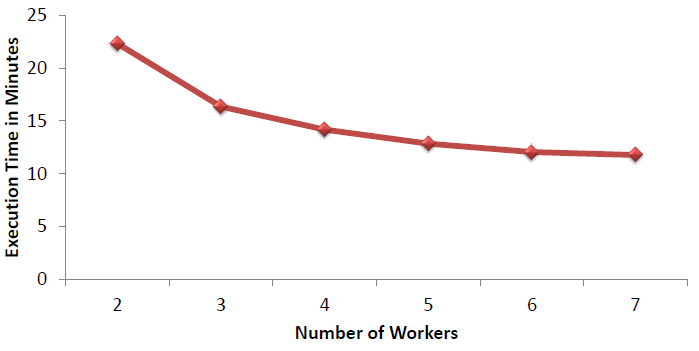
\includegraphics[scale=0.80]{improved_runtime}
	\caption{Improved Execution Time for processing \(10^5\) documents, Topics (K) = 90, Iterations = 20, Vocabulary Size = 137462, Total Document Pairs Classified =  4999950000}
	\label{fig: result_improved_runtime}
\end{figure}


\begin{figure}[htbp]
	\centering
		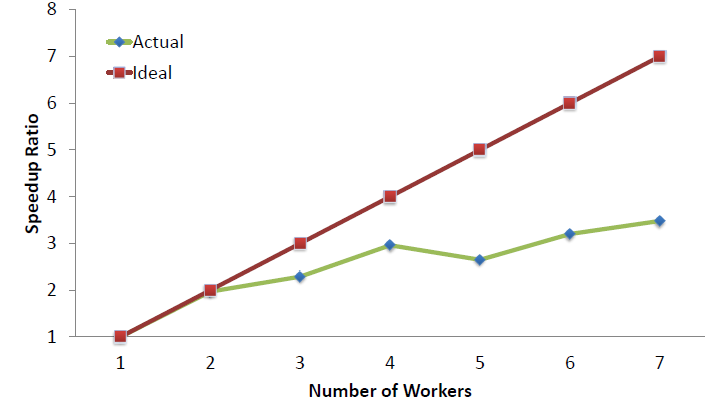
\includegraphics[scale=0.80]{speedup}
	\caption{Speedup for dataset size \(10^5\), Topics (K) = 90, Iterations = 20, Vocabulary Size = 137462, Total Document Pairs Classified =  4999950000}
	\label{fig: result_speedup}
\end{figure}

\begin{figure}[htbp]
	\centering
		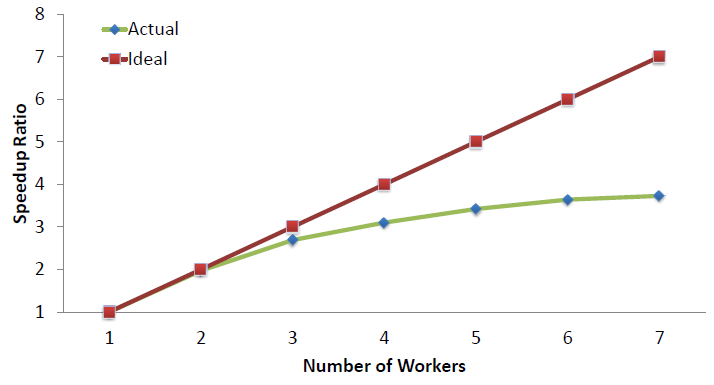
\includegraphics[scale=0.80]{improved_speedup}
	\caption{Improved Speedup for dataset size \(10^5\), Topics (K) = 90, Iterations = 20, Vocabulary Size = 137462, Total Document Pairs Classified =  4999950000}
	\label{fig: result_improved_speedup}
\end{figure}

\begin{figure}[htbp]
	\centering
		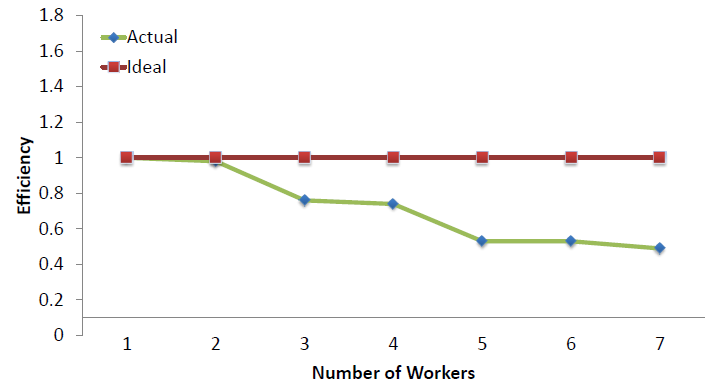
\includegraphics[scale=0.80]{Efficiency}
	\caption{Efficiency for dataset size \(10^5\), Topics (K) = 90, Iterations = 20, Vocabulary Size = 137462, Total Document Pairs Classified =  4999950000}
	\label{fig: result_efficiency}
\end{figure}

\begin{figure}[htbp]
	\centering
		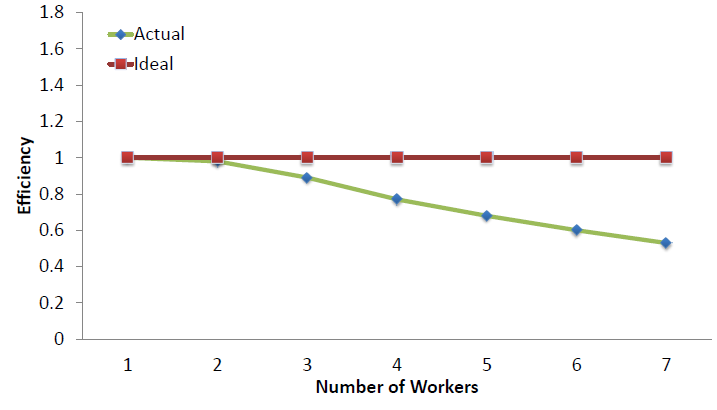
\includegraphics[scale=0.80]{improved_Efficiency}
	\caption{Improved Efficiency for dataset size \(10^5\), Topics (K) = 90, Iterations = 20, Vocabulary Size = 137462, Total Document Pairs Classified =  4999950000}
	\label{fig: result_improved_efficiency}
\end{figure}


\par Based on the execution time of the Semantic Document Matching process, the speedup and efficiency of the approach are calculated as per the evaluation metrics discussed in \ref{section: evaluation}. The results obtained on calculating efficiency and speed up can be observed in \ref{fig: result_speedup} and \ref{fig: result_efficiency}. We only ran 20 iterations on the input dataset as our primary focus is to increase the efficiency of the implementation but not calculating the convergence. As the execution time of the implementation has improved after performing optimizations, we have the improved speedup and efficiency for the same dataset and parameters respectively. The improved speedup and efficiency can be observed in \ref{fig: result_improved_speedup} and \ref{fig: result_improved_efficiency} respectively.

\subsection{Evaluating Threshold based Classification}
\label{subsection: evaluating threshold}

From \ref{fig: result_runtime_classification}, we can observe the total runtime taken by the document matching process for different datasets using a cluster with 7 worker nodes. To process \(10^4\) documents, on an average it took 7 minutes for the cluster to classify the documents and the execution time is increased for processing \(10^5\) documents to 13 minutes. The execution time taken to process \(10^5\) documents got faster when compared to the execution time taken to process \(10^4\) documents. This is due to only a few executors were assigned for the tasks by the YARN cluster manager for processing smaller datasets where as every worker was assigned a job in processing \(10^5\) documents. From \ref{tab:document pairs classified by threshold based classification}, we can observe the total number of document pairs classified based on the threshold value in the classification stage.

\begin{figure}[htbp]
	\centering
		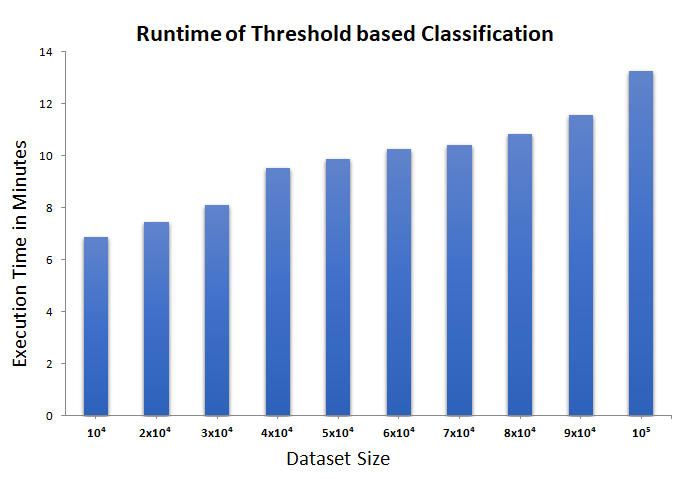
\includegraphics[scale=0.80]{runtime_threshold_classification}
	\caption{Runtime of Threshold based Classification for varying datasets}
	\label{fig: result_runtime_classification}
\end{figure}

\begin{table}[htbp]
	\centering
		\begin{tabular}{cc}\toprule
		Number of Documents in Input Dataset & Total Document Pairs Classified\\\midrule
		\(10^4\) & 49995000 \\\addlinespace 
		\(2*10^4\)  &  199990000 \\\addlinespace
        \(3*10^4\)  &  449985000 \\\addlinespace
        \(4*10^4\)  &  799980000 \\\addlinespace
        \(5*10^4\)  &  1249975000 \\\addlinespace
        \(6*10^4\)  &  1799970000 \\\addlinespace
        \(7*10^4\)  &  2449965000 \\\addlinespace
        \(8*10^4\)  &  3199960000\\\addlinespace
        \(9*10^4\)  &  4049955000 \\\addlinespace
        \(10^5\)  &  4999950000 \\\bottomrule
		\end{tabular}
	\caption{A Table illustrating document pairs classified by threshold based classification}
	\label{tab:document pairs classified by threshold based classification}
\end{table}


\subsection{Evaluating Effectiveness}
\label{subsection: evaluating effectiveness}

The aim of this evaluation is to verify and compare the quality of the results obtained from the Semantic Document Matching process with the generated golden data. On comparing the results obtained from classification stage to the golden data, We have evaluated this experiment by classifying the obtained results as true positives, true negatives, false positives, and false negatives in the evaluation stage. Based on these classifications, the quality measures like precision, recall, and f-measure are calculated for the input dataset consisting of \(10^4\) documents. The results of precision, recall, and f-measure are illustrated in \ref{tab:fmeasure}. 

\begin{table}[htbp]
	\centering
		\begin{tabular}{cccc}\toprule
		Number of Documents in Input Dataset & Precision & Recall & F-measure\\\midrule
		
        \(10^4\)  &  0.366 & 0.168 & 0.230 \\\bottomrule
		\end{tabular}
	\caption{A Table illustrating Effectiveness measures}
	\label{tab:fmeasure}
\end{table}

\subsection{Discussions}
\label{section: Discussions}

\textbf{Speedup and Efficiency}

\par From \ref{fig: result_runtime}, we can observe that the execution time is reduced rapidly as the number of worker nodes increased but then suddenly increased. On analyzing we found that the increase of execution time occurred because the input data is not distributed equally to all the worker nodes in the cluster. Hence we have performed the following optimizations to achieve better efficiency

\begin{itemize}
\item The default Java serialization is changed to kryo serializer which helps in faster serialization as per the official apache spark suggestion \cite{spark:website}.
\item With the help of repartition() method, the data is distributed equally among all the worker nodes in the cluster by specifying the number of partitions. The method is invoked every time when the data is loaded into a DataFrame using Spark SQL. The number of partitions is specified in proportion to the number of cores that are set while executing the implementation process.
\end{itemize}

\par Usually it takes \(O(n^2)\) computations to perform document pair comparison. However by defining a join condition as discussed in \ref{implement: Document Pair Comparison}, we have achieved the good results in reducing the number of computations required in comparing the document pairs and is illustrated in \ref{fig: result_runtime_classification}.

\par Though we have achieved some improvement in increasing the efficiency of the Semantic Document Matching process on applying the above optimizations, but are not appreciable when compared to the ideal efficiency and speedup and the same can be observed from \ref{fig: result_improved_efficiency} and \ref{fig: result_improved_speedup}. In general, the ideal efficiency achieved should be constant with the increase of worker nodes in the cluster. But the efficiency we have obtained for our approach is dropped with the increase of worker nodes in the cluster. We analyze that the reason for the loss of efficiency is due to heterogeneous nature of the cluster. At the driver node, most of the time is lost in waiting for some of the executors in the completion of tasks as the heavy computations need to be performed for generating the similarity score for two documents.




\textbf{Effectiveness}

From \ref{tab:fmeasure}, we can observe that the accuracy obtained by the Semantic Document Matching process is very poor. We analyze the following are major reasons for poor accuracy:

\begin{itemize}
\item The focus of the thesis is primarily on increasing the efficiency of the implemented process. As a result, the perplexity of the LDA modeling techniques and model fitting was not measured because the efficiency degrades with the increase in accuracy of the output data.

\item As discussed in earlier sections, the input dataset rcv1 do not provide any information on ground truth representing the similarity between two documents. Therefore, we have designed a workaround method and is discussed in \ref{implement:evaluation} to generate golden data. But we observed that the implemented workaround method is still not perfect as some of the labels generated in golden data contain null values as some of the documents in rcv1 do not possess the topic information. The presence of null values decreases the accuracy.
\end{itemize}

\par The workaround method was not improved further due to the limitation of thesis period. The semantic similarity obtained by the Document Matching process speaks about how two documents are semantically similar but the golden data represents only about the overlap of topics between two documents. Hence, the results obtained cannot be compared to golden data. But we have presented the results to address the existing problems in calculating the accuracy.

%Die Beurteilung ist einer der wichtigsten Abschnitte der Arbeit
%- Sie enthält die Quintessenz des gesamten Projektes
%Viele lesen nur die Einführung und die Beurteilung an
%- Hier muss also alles Wichtige drin stehen!
%Hier beweisen Sie dass Sie …
%- die Aufgabe und deren Bedeutung verstanden haben
%- die Ergebnisse richtig zu interpretieren vermögen
%- wissen, worauf es bei diese Arbeit ankam


\ifgerman{\chapter{Zusammenfassung}}{\chapter{Conclusion}}
\label{conclusion}

In this thesis, we designed and implemented an approach to match documents based on their semantic similarity with in the corpus. To efficiently process the huge amount of documents, this thesis is implemented in a parallel processing environment using the Apache Spark framework. The semantic similarity between the documents is measured by discovering the topics from each document. The approach is implemented as a combination of Spark SQL, DataFrames API and machine learning components with in the Apache Spark framework. The designed and implemented approach consists of 6 stages namely pre-processing stage, count vectorization, Latent Dirichlet Allocation (LDA) modeling, Document Pair comparison, classification and evaluation stages.

\par As our primary focus is to increase the efficiency, We have evaluated the speedup and efficiency of the implemented approach using various experiments. For evaluating the efficiency, different sizes of the input dataset and the number of worker nodes are varied. As the approach is implemented in a parallel environment, the total execution time taken by the approach in obtaining the results is calculated. Based on the runtime obtained, speedup and efficiency are calculated. Further, we have improved the speedup and efficiency of the implementation approach by applying different optimization techniques. With the implemented approach, we also reduced the number of required computations  to less than \(O(n^2)\) computations for Document pair comparison. However, the implemented approach can only be applicable to match documents for macro level analysis i.e. calculating semantic similarity between documents by considering the structure of the document as a whole. Moreover, the efficiency of the implemented approach can further be improved either by adding more worker nodes in a cluster or by introducing more advanced optimization techniques.

Additionally, we calculated the effectiveness of the implementation to verify the quality of the results obtained. As the input dataset do not provide the golden data, we designed a workaround method and the golden data is generated to calculate the effectiveness by calculating precision, recall, and f-measure.
\ifgerman{\chapter{Zukunftige Arbeiten}}{\chapter{Future Work}}
\label{futurework}

In this chapter, we discuss the possible area of interests where this thesis can be extended. The following are the some of the directions for improving or extending this thesis:



\begin{itemize}
\item As we have designed and implemented the process on a macro level or document level i.e. the semantic similarity is calculated by considering the structure of the document as a whole, this thesis can be extended to process the documents at a micro level. At the micro level, the similarity can be carried out either at paragraph level or at a sentence level.

\item As Latent Dirichlet Allocation (LDA) is sensitive to the input data, the thesis can be extended to improve the input data quality by introducing more natural language processing techniques namely parts of speech detection, stemming, lemmatization etc as filters along with the existing pre-processing stages.

\item Latent Dirichlet Allocation techniques can be extended by implementing other inference algorithms and runtime can be compared with this thesis.

\item This thesis also can be extended in terms of improving the effectiveness of the input dataset used.
\end{itemize}






%*********************************************************************%
% APPENDIX                                                            %
%*********************************************************************%

%\appendix
%\include{chapters/appendix}

%*********************************************************************%
% LITERATURE                                                          %
%*********************************************************************%

\cleardoublepage
\phantomsection
\addcontentsline{toc}{chapter}{\bibname} % 
\bibliographystyle{IEEEtran} % plain gerplain abbrvnat unsrtnat alphag alpha
% in a thesis you have space... use full names
\bibliography{literature/Dharani}
% in a paper, space is limited. use abreviations
%\bibliography{../literature/IEEEabrv,../literature/MYabrv,../literature/literature}

%*********************************************************************%
% ERKLÄRUNG                                                           %
%*********************************************************************%

\ifnotdraft{
	\cleardoublepage
	\phantomsection
	\printindex
	%\thispagestyle{empty}
\vspace*{38\baselineskip}
\hbox to \textwidth{\hrulefill}
\par
Hiermit erkl\"are ich, dass ich die vorliegende Arbeit selbst\"andig verfasst und
keine anderen als die angegebenen Quellen und Hilfsmittel verwendet habe.

\signatureplace, den \signaturedate

%%%%%%%%%%%%%%%%%%%%%%%%%%%%%%%%%%%%%%%%%%%%%%%%%%%%%%%%%%%%%%%%%%%%%%%%
%% Hinweis:
%%
%% Diese Erklärung wird von der Prüfungsordnung für Diplomarbeiten 
%% verlangt und ist zu unterschreiben. Für Studienarbeiten ist diese
%% Erklärung nicht zwingend notwendig, schadet aber auch nicht.
%%%%%%%%%%%%%%%%%%%%%%%%%%%%%%%%%%%%%%%%%%%%%%%%%%%%%%%%%%%%%%%%%%%%%%%%
\clearpage

}

\end{document}
